% ============================================================
%  يُترجَم بـ XeLaTeX  (في Overleaf: Menu → Compiler → XeLaTeX)
%  الخط: Amiri (متوفر في Overleaf، أو حمّله من github.com/aliftype/amiri)
% ============================================================
\documentclass[12pt,a4paper]{article}
\usepackage[a4paper,margin=1.7cm,top=2.3cm,bottom=2.9cm,headheight=15pt,footskip=1.5cm]{geometry}
\usepackage{amsmath,amssymb}
\usepackage{icomma}
\usepackage[english,bidi=default,layout=lists]{babel}
\babelprovide[import,main]{arabic}
\babelfont{rm}[Scale=1.08]{Amiri}
\babelfont{sf}[Scale=1.08]{Amiri}
\usepackage[most]{tcolorbox}
\usepackage{tikz}
\usetikzlibrary{arrows.meta,calc,shadings}
\usepackage{array}
\usepackage{colortbl}
\usepackage{fancyhdr}
\usepackage{titlesec}
\usepackage{enumitem}
\usepackage{collcell}
\usepackage{needspace}
\usepackage{etoolbox}
\newcolumntype{C}{>{\collectcell\ar}c<{\endcollectcell}}
\pretocmd{\section}{\Needspace{15\baselineskip}}{}{}
\pretocmd{\subsection}{\Needspace{11\baselineskip}}{}{}

\definecolor{cDef}{HTML}{1F4E9C}
\definecolor{cThm}{HTML}{B3261E}
\definecolor{cRem}{HTML}{2E7D32}
\definecolor{cEx}{HTML}{C76B00}
\definecolor{cMeth}{HTML}{6A1B9A}
\definecolor{cSol}{HTML}{00695C}
\definecolor{cSec}{HTML}{1F3A68}

\titleformat{\section}{\Large\bfseries\color{cSec}}{\thesection.}{0.6em}{}[{\color{cSec!60}\titlerule[1pt]}]
\titleformat{\subsection}{\large\bfseries\color{cThm!85!black}}{\thesubsection.}{0.5em}{}
\titlespacing*{\section}{0pt}{14pt}{8pt}
\titlespacing*{\subsection}{0pt}{10pt}{5pt}
\setlength{\parindent}{0pt}
\setlength{\parskip}{4pt}
\setlist{itemsep=2pt,topsep=3pt}

\newtcolorbox{arbox}[3][]{enhanced,
  colback=#2!5,colframe=#2!80!black,arc=2mm,boxrule=0.8pt,
  left=6pt,right=6pt,top=8pt,bottom=5pt,
  fonttitle=\bfseries,coltitle=white,
  title={\foreignlanguage{arabic}{#3}},
  attach boxed title to top right={xshift=-5mm,yshift=-3mm},
  boxed title style={colback=#2!80!black,arc=1.5mm,boxrule=0pt},
  before upper={\selectlanguage{arabic}},
  before skip=8pt,after skip=8pt,breakable,#1}
\newenvironment{BOX}[2]{\begin{otherlanguage}{english}\begin{arbox}{#1}{#2}}{\end{arbox}\end{otherlanguage}}
\newenvironment{tarif}[1][تعريف]{\begin{BOX}{cDef}{#1}}{\end{BOX}}
\newenvironment{khassia}[1][خاصية]{\begin{BOX}{cThm}{#1}}{\end{BOX}}
\newenvironment{molahada}[1][ملاحظة]{\begin{BOX}{cRem}{#1}}{\end{BOX}}
\newenvironment{mithal}[1][مثال]{\begin{BOX}{cEx}{#1}}{\end{BOX}}
\newenvironment{tariqa}[1][طريقة]{\begin{BOX}{cMeth}{#1}}{\end{BOX}}

\newcounter{exo}
\newenvironment{tamrin}[1]{\stepcounter{exo}\begin{BOX}{cSec}{التمرين \theexo: #1}}{\end{BOX}}
\newenvironment{hal}{\Needspace{12\baselineskip}\begin{otherlanguage}{english}\begin{arbox}[breakable]{cSol}{حل التمرين \theexo}}{\end{arbox}\end{otherlanguage}}

\newenvironment{LTR}{\begin{otherlanguage}{english}}{\end{otherlanguage}}
\newcommand{\ar}[1]{\foreignlanguage{arabic}{#1}}

\renewcommand{\dots}{\mathinner{\ldotp\ldotp\ldotp}}
\renewcommand{\ldots}{\mathinner{\ldotp\ldotp\ldotp}}
\renewcommand{\cdots}{\mathinner{\cdotp\cdotp\cdotp}}
\newcommand{\N}{\mathbb{N}}
\newcommand{\Z}{\mathbb{Z}}
\newcommand{\D}{\mathbb{D}}
\newcommand{\Q}{\mathbb{Q}}
\newcommand{\R}{\mathbb{R}}
\newcommand{\pgcd}{\operatorname{PGCD}}
\newcommand{\ppcm}{\operatorname{PPCM}}

% \NLseg{a}{b}{[}{]} ; \NLright{a}{[} ; \NLleft{b}{]}  (interval on a number line)
\newcommand{\NLseg}[4]{\begin{LTR}\begin{tikzpicture}[baseline=-0.6ex]
 \draw[-{Stealth[length=2mm]},gray!70](0,0)--(3.4,0);
 \draw[line width=2pt,cThm!80!black](0.7,0)--(2.7,0);
 \node[cThm!80!black,font=\LARGE] at (0.7,0){$#3$};
 \node[cThm!80!black,font=\LARGE] at (2.7,0){$#4$};
 \node[below=3pt,font=\footnotesize] at (0.7,0){$#1$};
 \node[below=3pt,font=\footnotesize] at (2.7,0){$#2$};
\end{tikzpicture}\end{LTR}}
\newcommand{\NLright}[2]{\begin{LTR}\begin{tikzpicture}[baseline=-0.6ex]
 \draw[-{Stealth[length=2mm]},gray!70](0,0)--(3.4,0);
 \draw[line width=2pt,cThm!80!black](1.3,0)--(3.3,0);
 \node[cThm!80!black,font=\LARGE] at (1.3,0){$#2$};
 \node[below=3pt,font=\footnotesize] at (1.3,0){$#1$};
\end{tikzpicture}\end{LTR}}
\newcommand{\NLleft}[2]{\begin{LTR}\begin{tikzpicture}[baseline=-0.6ex]
 \draw[-{Stealth[length=2mm]},gray!70](0,0)--(3.4,0);
 \draw[line width=2pt,cThm!80!black](0.05,0)--(2.1,0);
 \node[cThm!80!black,font=\LARGE] at (2.1,0){$#2$};
 \node[below=3pt,font=\footnotesize] at (2.1,0){$#1$};
\end{tikzpicture}\end{LTR}}

% ---------- social-media icons (pure TikZ) ----------
\definecolor{cFB}{HTML}{1877F2}
\definecolor{cTG}{HTML}{229ED9}
\definecolor{cIG1}{HTML}{FEDA75}
\definecolor{cIG2}{HTML}{D62976}
\definecolor{cIG3}{HTML}{4F5BD5}
\newcommand{\fbicon}{\begin{LTR}\begin{tikzpicture}[baseline=-0.75ex,x=1em,y=1em]
 \fill[cFB] (0,0) circle (0.55);
 \node[white,inner sep=0,font=\usefont{TU}{lmss}{bx}{n}\small] at (0.04,-0.02) {f};
\end{tikzpicture}\end{LTR}}
\newcommand{\igicon}{\begin{LTR}
\begin{tikzpicture}[baseline=-0.75ex,x=1em,y=1em]
 \shade[lower left=cIG1,lower right=cIG2,upper left=cIG2,upper right=cIG3,rounded corners=0.28em] (-0.55,-0.55) rectangle (0.55,0.55);
 \draw[white,line width=0.09em,rounded corners=0.18em] (-0.36,-0.36) rectangle (0.36,0.36);
 \draw[white,line width=0.09em] (0,0) circle (0.17);
 \fill[white] (0.22,0.22) circle (0.05);
\end{tikzpicture}\end{LTR}}
\newcommand{\tgicon}{\begin{LTR}
\begin{tikzpicture}[baseline=-0.75ex,x=1em,y=1em]
 \fill[cTG] (0,0) circle (0.55);
 \fill[white] (-0.33,0.0) -- (0.32,0.27) -- (0.2,-0.3) -- (0.0,-0.15) -- (-0.08,-0.28) -- (-0.08,-0.08) -- cycle;
 \fill[cTG!70!black] (-0.08,-0.08) -- (0.25,0.2) -- (0.0,-0.15) -- (-0.08,-0.28) -- cycle;
\end{tikzpicture}\end{LTR}}
% page number: black box, white two-digit number, at the right of the social row
\newcommand{\PageBox}{\begin{LTR}\tikz[baseline=(p.base)]\node[fill=black,text=white,inner sep=2.5pt,minimum width=1.6em,minimum height=1.3em,font=\usefont{TU}{lmss}{bx}{n}\small](p){\ifnum\value{page}<10 0\fi\arabic{page}};\end{LTR}}
% visual left-to-right order: Telegram | Instagram | Facebook | page box
\newcommand{\SocialRow}{\begin{otherlanguage}{english}%
 \ar{\textbf{الأستاذ سوايسية هشام للرياضيات}}\ \tgicon\hfill
 \textbf{prof\_hicham\_math}\ \igicon\hfill
 \ar{\textbf{الأستاذ سوايسية هشام للرياضيات}}\ \fbicon\hspace{2.2em}\PageBox\end{otherlanguage}}

\pagestyle{fancy}
\fancyhf{}
\renewcommand{\headrulewidth}{0.6pt}
\renewcommand{\footrulewidth}{0.4pt}
% \SetHeader{right head: document title}{left head: level -- stream}
\newcommand{\SetHeader}[2]{%
 \fancyhead[C]{\parbox{\textwidth}{\ar{#1\hfill #2}}}%
 \fancyfoot[C]{\parbox{\textwidth}{\small\SocialRow}}}
\usepackage{tkz-tab}
\usepackage{multicol}
% variation / sign table (LTR)
\newenvironment{TAB}{\par\begin{center}\begin{LTR}\begin{tikzpicture}[scale=0.95,every node/.style={font=\small}]}{\end{tikzpicture}\end{LTR}\end{center}}
% grid + axes, clipped: \begin{GR}{xmin}{xmax}{ymin}{ymax}{unit cm}
\newenvironment{GR}[5]{\par\begin{center}\begin{LTR}\begin{tikzpicture}[x=#5cm,y=#5cm,font=\footnotesize]
 \draw[gray!25,very thin] (#1,#3) grid (#2,#4);
 \draw[-{Stealth[length=2mm]}] (#1,0)--(#2+0.3,0) node[below left]{$x$};
 \draw[-{Stealth[length=2mm]}] (0,#3)--(0,#4+0.3) node[below left]{$y$};
 \node[below left] at (0,0){$O$};
 \begin{scope}\clip (#1,#3) rectangle (#2,#4);}
{\end{scope}\end{tikzpicture}\end{LTR}\end{center}}
\newcommand{\Ticks}[2]{\foreach \t in {#1} \node[below,font=\scriptsize] at (\t,0){$\t$}; \foreach \t in {#2} \node[left,font=\scriptsize] at (0,\t){$\t$};}
\newcommand{\bx}[1]{\ensuremath{\colorbox{cDef!12}{$\displaystyle #1$}}}
\newcommand{\TwoCol}[4]{\par\begin{LTR}\noindent\begin{minipage}[t]{#1\textwidth}\selectlanguage{arabic}#2\end{minipage}\hfill\begin{minipage}[t]{#3\textwidth}\selectlanguage{arabic}#4\end{minipage}\end{LTR}\par}
\newcommand{\RL}[4]{\TwoCol{#3}{#4}{#1}{#2}}  % \RL{w1}{right content}{w2}{left content}
\newcommand{\ok}{$\textcolor{cRem}{\checkmark}$}
\newcommand{\limn}{\displaystyle\lim_{n\to+\infty}}
% sub-questions, each on its own line
\newenvironment{sq}{\begin{itemize}[leftmargin=2.4em,itemsep=3pt]}{\end{itemize}}
\newcommand{\qa}{\item[(أ)]}\newcommand{\qb}{\item[(ب)]}\newcommand{\qc}{\item[(جـ)]}\newcommand{\qd}{\item[(د)]}\newcommand{\qe}{\item[(هـ)]}
\newcommand{\pa}{\par\smallskip\textbf{(أ)} }\newcommand{\pb}{\par\smallskip\textbf{(ب)} }\newcommand{\pc}{\par\smallskip\textbf{(جـ)} }\newcommand{\pd}{\par\smallskip\textbf{(د)} }\newcommand{\pe}{\par\smallskip\textbf{(هـ)} }
\newcommand{\QQ}[1]{\par\smallskip\textbf{#1.} }
\newenvironment{tmr}{\stepcounter{exo}\begin{BOX}{cSec}{تمرين محلول \theexo}}{\end{BOX}}
\newcommand{\ABC}[3]{\\[2pt]\begin{tabular}{p{0.28\textwidth}p{0.28\textwidth}p{0.28\textwidth}}(جـ) \ #3 & (ب) \ #2 & (أ) \ #1\end{tabular}}
\pretocmd{\section}{\Needspace{24\baselineskip}}{}{}
\newtcbox{\bxtbox}{on line,colback=cDef!12,colframe=cDef!12,boxrule=0pt,arc=1pt,boxsep=0pt,left=2pt,right=2pt,top=1pt,bottom=1pt}
\newcommand{\bxt}[1]{\foreignlanguage{english}{\bxtbox{\ar{#1}}}}
\SetHeader{\small\bfseries\color{cSec}ملخص: النهايات والاستمرارية والاشتقاقية}{\small\color{cSec}السنة الثالثة ثانوي -- الشعب العلمية}
\let\origNeedspace\Needspace
\renewcommand{\Needspace}[1]{\origNeedspace{14\baselineskip}}
\newcommand{\Lim}[1]{\lim\limits_{#1}}
\begin{document}
\begin{LTR}
\begin{tcolorbox}[enhanced,colback=cSec,colframe=cSec,arc=3mm,halign=center,boxrule=0pt,top=12pt,bottom=12pt,before upper={\selectlanguage{arabic}}]
{\color{white}\fontsize{25}{32}\selectfont\bfseries النهايات والاستمرارية والاشتقاقية}\\[8pt]
{\color{white}\large ملخص شامل مع أمثلة وأشكال وتمارين محلولة خطوة بخطوة}\\[5pt]
{\color{white}\large السنة الثالثة ثانوي -- علوم تجريبية، رياضيات، تقني رياضي}
\end{tcolorbox}
\end{LTR}

\begin{BOX}{cSec}{محتوى الملخص}
\begin{enumerate}[label=\textbf{\arabic*.}]
\item تذكير: إشارة $ax+b$ وثلاثي الحدود، تحليل كثير حدود، الزوجية والفردية، عناصر التناظر، تمثيلات مستنتجة.
\item النهايات: نهاية منتهية وغير منتهية عند $\pm\infty$ وعند عدد، النهاية من اليمين ومن اليسار، العمليات، حالات عدم التعيين وطرق إزالتها، نهاية دالة مركبة، النهايات المثلثية، المقارنة والحصر.
\item السلوك التقاربي: المستقيمات المقاربة (أفقي، عمودي، مائل)، الوضع النسبي، المنحنيات المتقاربة، قراءة بيانية.
\item الاستمرارية: التعريف، الدوال المألوفة، القراءة البيانية، مبرهنة القيم المتوسطة ونتيجتها، الحصر بالتنصيف وبالمسح، صورة مجال.
\item الاشتقاقية: العدد المشتق، المماس، الاشتقاق من اليمين ومن اليسار، نصف المماس والنقطة الزاوية، التقريب التآلفي، المشتقات والعمليات، مشتق دالة مركبة، المشتقات المتتابعة.
\item الدوال المثلثية $x\mapsto\cos(\omega x+\varphi)$ و $x\mapsto\sin(\omega x+\varphi)$: المشتقة، الدور، الدراسة على مجال طوله الدور، التمثيل البياني.
\item المعادلات التفاضلية من الشكل $y'=f$ حيث $f$ دالة مألوفة.
\item دراسة دالة: اتجاه التغير، القيم الحدية، نقطة الانعطاف، المناقشة البيانية $f(x)=m$.
\item حل مشكلات بتوظيف المشتقات: الاستمثال (أكبر قيمة، أصغر قيمة).
\item أخطاء شائعة، تمارين محلولة، ثم خلاصة الطرائق.
\end{enumerate}
\end{BOX}
%================================================================
\section{تذكير ضروري}
\subsection{إشارة $ax+b$ \ ($a\neq0$) وإشارة ثلاثي الحدود}
\begin{khassia}[إشارة $ax+b$]
$ax+b=0\iff x=-\dfrac{b}{a}$. \ إشارة $ax+b$ هي \textbf{عكس إشارة $a$} على يسار $-\frac{b}{a}$ و\textbf{إشارة $a$} على يمينه:
\begin{TAB}
\tkzTabInit[lgt=2.4,espcl=3.2]{$x$/1,$ax+b$/1}{$-\infty$,$-\frac{b}{a}$,$+\infty$}
\tkzTabLine{,\hbox{\ar{عكس إشارة $a$}},z,\hbox{\ar{إشارة $a$}},}
\end{TAB}
\end{khassia}

\begin{khassia}[إشارة $ax^{2}+bx+c$ \ ($a\neq0$) حسب المميز $\Delta=b^{2}-4ac$]
\begin{itemize}
\item $\Delta>0$: جذران $x_1=\dfrac{-b-\sqrt{\Delta}}{2a}$ و $x_2=\dfrac{-b+\sqrt{\Delta}}{2a}$؛ التحليل $a(x-x_1)(x-x_2)$؛ الإشارة: \textbf{إشارة $a$ خارج الجذرين وعكسها بينهما}.
\item $\Delta=0$: جذر مضاعف $x_0=-\dfrac{b}{2a}$؛ التحليل $a(x-x_0)^{2}$؛ الإشارة: إشارة $a$ (وتنعدم عند $x_0$).
\item $\Delta<0$: لا جذور ولا تحليل؛ الإشارة: \textbf{إشارة $a$} على $\R$.
\end{itemize}
\end{khassia}

\subsection{تحليل كثير حدود}
\begin{khassia}
إذا كان $\alpha$ جذرًا لكثير الحدود $P$ (أي $P(\alpha)=0$) فإنه يوجد كثير حدود $Q$ درجته أقل بواحد من درجة $P$ حيث: \bx{P(x)=(x-\alpha)\,Q(x)}.\par
نعيّن $Q$ بالمطابقة، أو بالقسمة الإقليدية، أو بطريقة هورنر.
\end{khassia}

\begin{mithal}[$P(x)=x^{3}-x^{2}-4x+4$]
$P(2)=8-4-8+4=0$، إذن نكتب:
\[ P(x)=(x-2)(ax^{2}+bx+c)=ax^{3}+(b-2a)x^{2}+(c-2b)x-2c. \]
بالمطابقة: $a=1$ ، $b-2a=-1$ ، $-2c=4$، ومنه $a=1$ ، $b=1$ ، $c=-2$:
\[ \bx{P(x)=(x-2)(x^{2}+x-2)=(x-2)(x-1)(x+2)} \]
\textbf{بطريقة هورنر} (معاملات $P$ ثم الجذر $2$):
\begin{center}
\renewcommand{\arraystretch}{1.25}
\begin{tabular}{|C|c|c|c|c|}\hline
\rowcolor{cSec!12} معاملات $P$ & $1$ & $-1$ & $-4$ & $4$\\\hline
$\alpha=2$ & & $2$ & $2$ & $-4$\\\hline
معاملات $Q$ & $1$ & $1$ & $-2$ & $0$\\\hline
\end{tabular}
\end{center}
\end{mithal}

\subsection{الدالة الزوجية والدالة الفردية}
\begin{tarif}
$f$ دالة مجموعة تعريفها $D_f$ متناظرة بالنسبة إلى $0$ (من أجل كل $x\in D_f$: $-x\in D_f$).
\begin{itemize}
\item $f$ \textbf{زوجية} إذا كان $f(-x)=f(x)$: منحناها متناظر بالنسبة إلى \textbf{محور التراتيب}.
\item $f$ \textbf{فردية} إذا كان $f(-x)=-f(x)$: منحناها متناظر بالنسبة إلى \textbf{المبدأ} $O$.
\end{itemize}
\end{tarif}
\begin{mithal}
$f(x)=\dfrac{2x^{2}}{x^{2}-4}$ على $\R-\{-2;2\}$: $f(-x)=\dfrac{2(-x)^{2}}{(-x)^{2}-4}=f(x)$، إذن $f$ \bxt{زوجية}.\par
$g(x)=x^{3}-x$ على $\R$: $g(-x)=-x^{3}+x=-g(x)$، إذن $g$ \bxt{فردية}.
\end{mithal}

\subsection{مركز تناظر ومحور تناظر}
\begin{khassia}
\begin{itemize}
\item النقطة $\Omega(\alpha;\beta)$ \textbf{مركز تناظر} لـ $(C_f)$ يكافئ: من أجل كل $x\in D_f$:\par
\hfill $(2\alpha-x)\in D_f$ \quad و \quad \bx{f(2\alpha-x)+f(x)=2\beta}\hfill\null
\item المستقيم ذو المعادلة $x=\alpha$ \textbf{محور تناظر} لـ $(C_f)$ يكافئ: من أجل كل $x\in D_f$:\par
\hfill $(2\alpha-x)\in D_f$ \quad و \quad \bx{f(2\alpha-x)=f(x)}\hfill\null
\end{itemize}
\end{khassia}
\begin{mithal}
$f(x)=x+2+\dfrac{3}{x-1}$ على $\R-\{1\}$: إذا كان $x\neq1$ فإن $2-x\neq1$، و
\[ f(2-x)+f(x)=(2-x)+2+\frac{3}{1-x}+x+2+\frac{3}{x-1}=6=2\times3, \]
إذن $\Omega(1;3)$ \bxt{مركز تناظر للمنحنى $(C_f)$}.
\end{mithal}

\subsection{تمثيلات بيانية مستنتجة من $(C_f)$}
\begin{khassia}
\begin{itemize}
\item $g(x)=f(x+b)+k$: $(C_g)$ صورة $(C_f)$ بالانسحاب الذي شعاعه $\vec{u}\begin{pmatrix}-b\\ k\end{pmatrix}$.
\item $g(x)=-f(x)$: $(C_g)$ نظير $(C_f)$ بالنسبة إلى محور الفواصل.
\item $g(x)=f(-x)$: $(C_g)$ نظير $(C_f)$ بالنسبة إلى محور التراتيب.
\item $g(x)=|f(x)|$: $(C_g)$ ينطبق على $(C_f)$ حيث $f(x)\geqslant0$، ونظيره بالنسبة إلى محور الفواصل حيث $f(x)\leqslant0$.
\item $g(x)=f(|x|)$: $(C_g)$ ينطبق على $(C_f)$ من أجل $x\geqslant0$، ونكمل بالتناظر بالنسبة إلى محور التراتيب ($g$ زوجية).
\end{itemize}
\end{khassia}
\begin{mithal}[$f(x)=x^{2}-2x-1$ و $g(x)=|f(x)|$]
الجزء من $(C_f)$ الواقع تحت محور الفواصل (بين $1-\sqrt2$ و $1+\sqrt2$) نرسم نظيره بالنسبة إلى محور الفواصل، والباقي يبقى كما هو.
\begin{GR}{-2}{4}{-2.5}{4}{0.7}
\Ticks{-1,1,2,3}{-2,-1,1,2,3}
\draw[cDef,thick,dashed,domain=-1.8:3.8,samples=80] plot(\x,{\x*\x-2*\x-1});
\draw[cThm,very thick,domain=-1.8:-0.4142,samples=40] plot(\x,{\x*\x-2*\x-1});
\draw[cThm,very thick,domain=-0.4142:2.4142,samples=60] plot(\x,{-(\x*\x-2*\x-1)});
\draw[cThm,very thick,domain=2.4142:3.8,samples=40] plot(\x,{\x*\x-2*\x-1});
\node[cDef] at (1,-2.3){$(C_f)$};
\node[cThm] at (3.4,3.6){$(C_g)$};
\end{GR}
\end{mithal}

%================================================================
\section{النهايات}
\subsection{النهاية عند $+\infty$ أو عند $-\infty$}
\begin{tarif}
\begin{itemize}
\item نقول إن $f$ تقبل النهاية $+\infty$ عند $+\infty$ إذا كان كل مجال من الشكل $]A;+\infty[$ يحوي كل القيم $f(x)$ من أجل $x$ كبير بالقدر الكافي. نكتب \bx{\Lim{x\to+\infty}f(x)=+\infty}.
\item نقول إن $f$ تقبل النهاية $\ell$ (عدد حقيقي) عند $+\infty$ إذا كان كل مجال مفتوح يشمل $\ell$ يحوي كل القيم $f(x)$ من أجل $x$ كبير بالقدر الكافي. نكتب \bx{\Lim{x\to+\infty}f(x)=\ell}.
\item نعرّف بنفس الطريقة النهايات عند $-\infty$ والنهاية $-\infty$.
\end{itemize}
\end{tarif}

\begin{khassia}[نهايات الدوال المرجعية ($n\in\N^{*}$)]
\begin{align*}
&\Lim{x\to+\infty}x^{n}=+\infty & &\Lim{x\to+\infty}\sqrt{x}=+\infty & &\Lim{x\to\pm\infty}\frac{1}{x^{n}}=0 & &\Lim{x\to+\infty}\frac{1}{\sqrt{x}}=0
\end{align*}
$\Lim{x\to-\infty}x^{n}=+\infty$ إذا كان $n$ زوجيًا، و $\Lim{x\to-\infty}x^{n}=-\infty$ إذا كان $n$ فرديًا.
\end{khassia}

\subsection{النهاية عند عدد حقيقي $a$ -- النهاية من اليمين ومن اليسار}
\begin{tarif}
\begin{itemize}
\item \bx{\Lim{x\to a}f(x)=+\infty}: تكون $f(x)$ أكبر من أي عدد $A$ عندما يكون $x$ قريبًا بالقدر الكافي من $a$.
\item \bx{\Lim{x\to a}f(x)=\ell}: تكون $f(x)$ قريبة من $\ell$ بالقدر الذي نريد عندما يكون $x$ قريبًا بالقدر الكافي من $a$.
\item نكتب $\Lim{x\to a^{+}}f(x)$ (أو $\Lim{\substack{x\to a\\ x>a}}f(x)$) للنهاية \textbf{من اليمين}، و $\Lim{x\to a^{-}}f(x)$ (أو $\Lim{\substack{x\to a\\ x<a}}f(x)$) للنهاية \textbf{من اليسار}.
\item تقبل $f$ نهاية عند $a$ إذا وفقط إذا كانت النهايتان من اليمين ومن اليسار موجودتين ومتساويتين.
\end{itemize}
\end{tarif}

\begin{mithal}[$f(x)=\dfrac{1}{x-2}$ عند $2$]
\RL{0.5}{
$\Lim{x\to2^{+}}(x-2)=0^{+}$، إذن \bx{\Lim{x\to2^{+}}\frac{1}{x-2}=+\infty}.\par
$\Lim{x\to2^{-}}(x-2)=0^{-}$، إذن \bx{\Lim{x\to2^{-}}\frac{1}{x-2}=-\infty}.\par
النهايتان مختلفتان: $f$ لا تقبل نهاية عند $2$.\par
وعند $\pm\infty$: $\Lim{x\to\pm\infty}\frac{1}{x-2}=0$.
}{0.46}{
\begin{GR}{-1}{5}{-3}{3}{0.6}
\Ticks{1,2,3,4}{-2,-1,1,2}
\draw[cRem,thick,dashed] (2,-3)--(2,3);
\draw[cDef,very thick,domain=-1:1.67,samples=60] plot(\x,{1/(\x-2)});
\draw[cDef,very thick,domain=2.34:5,samples=60] plot(\x,{1/(\x-2)});
\node[cRem,font=\scriptsize] at (2.6,2.7){$x=2$};
\end{GR}
}
\end{mithal}

\subsection{العمليات على النهايات}
\begin{khassia}[نهاية المجموع $f+g$]
\begin{center}\renewcommand{\arraystretch}{1.3}
\begin{tabular}{|c|C|C|C|C|C|C|}\hline
\rowcolor{cSec!12}$\lim f$ & $\ell$ & $\ell$ & $\ell$ & $+\infty$ & $-\infty$ & $+\infty$\\\hline
$\lim g$ & $\ell'$ & $+\infty$ & $-\infty$ & $+\infty$ & $-\infty$ & $-\infty$\\\hline
$\lim (f+g)$ & $\ell+\ell'$ & $+\infty$ & $-\infty$ & $+\infty$ & $-\infty$ & \textbf{ح.ع.ت}\\\hline
\end{tabular}\end{center}
\end{khassia}
\begin{khassia}[نهاية الجداء $f\times g$]
\begin{center}\renewcommand{\arraystretch}{1.3}
\begin{tabular}{|c|C|C|C|C|}\hline
\rowcolor{cSec!12}$\lim f$ & $\ell$ & $\ell\neq0$ & $0$ & $\infty$\\\hline
$\lim g$ & $\ell'$ & $\infty$ & $\infty$ & $\infty$\\\hline
$\lim (f\times g)$ & $\ell\times\ell'$ & $\infty$ & \textbf{ح.ع.ت} & $\infty$\\\hline
\end{tabular}\end{center}
الإشارة ($+\infty$ أو $-\infty$) تُحدَّد بقاعدة إشارات الجداء.
\end{khassia}
\begin{khassia}[نهاية حاصل القسمة $\dfrac{f}{g}$]
\begin{center}\renewcommand{\arraystretch}{1.3}
\begin{tabular}{|c|C|C|C|C|C|C|}\hline
\rowcolor{cSec!12}$\lim f$ & $\ell$ & $\ell$ & $\ell\neq0$ & $0$ & $\infty$ & $\infty$\\\hline
$\lim g$ & $\ell'\neq0$ & $\infty$ & $0^{+}$ أو $0^{-}$ & $0$ & $\ell'$ & $\infty$\\\hline
$\lim \frac{f}{g}$ & $\frac{\ell}{\ell'}$ & $0$ & $\infty$ & \textbf{ح.ع.ت} & $\infty$ & \textbf{ح.ع.ت}\\\hline
\end{tabular}\end{center}
الإشارة تُحدَّد بقاعدة الإشارات؛ لذلك نحدد دائمًا هل المقام يؤول إلى $0^{+}$ أو إلى $0^{-}$.
\end{khassia}

\begin{molahada}[حالات عدم التعيين (ح.ع.ت) الأربع]
\[ \bx{+\infty-\infty} \qquad \bx{0\times\infty} \qquad \bx{\frac{\infty}{\infty}} \qquad \bx{\frac{0}{0}} \]
في هذه الحالات لا نستطيع الاستنتاج مباشرة: يجب \textbf{تحويل العبارة} أولًا.
\end{molahada}

\subsection{كثيرات الحدود والدوال الناطقة عند $\pm\infty$}
\begin{khassia}
\begin{itemize}
\item نهاية كثير حدود عند $\pm\infty$ هي نهاية \textbf{حده الأعلى درجة}.
\item نهاية دالة ناطقة عند $\pm\infty$ هي نهاية \textbf{حاصل قسمة الحدين الأعلى درجة} في البسط والمقام.
\end{itemize}
\end{khassia}
\begin{mithal}
\begin{itemize}
\item $\Lim{x\to-\infty}\left(-2x^{3}+x^{2}+5\right)=\Lim{x\to-\infty}\left(-2x^{3}\right)=\bx{+\infty}$.
\item $\Lim{x\to+\infty}\dfrac{2x^{3}-x+1}{x^{2}+4}=\Lim{x\to+\infty}\dfrac{2x^{3}}{x^{2}}=\Lim{x\to+\infty}2x=\bx{+\infty}$.
\item $\Lim{x\to-\infty}\dfrac{3x^{2}-1}{2x^{2}+x}=\Lim{x\to-\infty}\dfrac{3x^{2}}{2x^{2}}=\bx{\dfrac{3}{2}}$ ؛ \quad $\Lim{x\to+\infty}\dfrac{x+5}{x^{3}-1}=\Lim{x\to+\infty}\dfrac{1}{x^{2}}=\bx{0}$.
\end{itemize}
\end{mithal}

%================================================================
\section{إزالة حالات عدم التعيين}
\subsection{الحالة $\dfrac{0}{0}$ عند عدد $a$}
\begin{tariqa}
\begin{itemize}
\item \textbf{كثيرات حدود:} $a$ جذر للبسط وللمقام، نحلل كلًّا منهما ونختزل $(x-a)$.
\item \textbf{جذر تربيعي:} نضرب البسط والمقام في \textbf{المرافق} ($\left(\sqrt{A}-B\right)\left(\sqrt{A}+B\right)=A-B^{2}$) ثم نختزل $(x-a)$.
\item \textbf{مقام من الشكل $x-a$ وبسط $g(x)-g(a)$:} نستعمل \textbf{العدد المشتق}: $\Lim{x\to a}\dfrac{g(x)-g(a)}{x-a}=g'(a)$.
\end{itemize}
\end{tariqa}

\begin{mithal}[التحليل]
\begin{itemize}
\item $\Lim{x\to2}\dfrac{-3x^{2}+4x+4}{x^{2}-5x+6}$: \ ح.ع.ت $\frac{0}{0}$. \ نحلل البسط والمقام ($2$ جذر لكل منهما):
\[ -3x^{2}+4x+4=(x-2)(-3x-2) \qquad\qquad x^{2}-5x+6=(x-2)(x-3) \]
\[ \Lim{x\to2}\frac{(x-2)(-3x-2)}{(x-2)(x-3)}=\Lim{x\to2}\frac{-3x-2}{x-3}=\frac{-8}{-1}=\bx{8}. \]
\item $\Lim{x\to-2}\dfrac{x^{3}+x^{2}-8x-12}{x^{3}+8}$: \ ح.ع.ت $\frac{0}{0}$. \ بالقسمة على $(x+2)$:
\[ \Lim{x\to-2}\frac{(x+2)(x^{2}-x-6)}{(x+2)(x^{2}-2x+4)}=\frac{4+2-6}{4+4+4}=\frac{0}{12}=\bx{0}. \]
\end{itemize}
\end{mithal}

\begin{mithal}[المرافق]
\begin{itemize}
\item $\Lim{x\to5}\dfrac{\sqrt{2x-1}-3}{x-5}$: \ ح.ع.ت $\frac{0}{0}$:
\[ \frac{\sqrt{2x-1}-3}{x-5}=\frac{(2x-1)-9}{(x-5)\left(\sqrt{2x-1}+3\right)}=\frac{2}{\sqrt{2x-1}+3}\ \xrightarrow[x\to5]{}\ \frac{2}{3+3}=\bx{\frac13}. \]
\item $\Lim{x\to2^{+}}\dfrac{\sqrt{x-2}}{x^{2}-2x}$: \ ح.ع.ت $\frac{0}{0}$. \ من أجل $x>2$: $x-2=\sqrt{x-2}\times\sqrt{x-2}$:
\[ \frac{\sqrt{x-2}}{x(x-2)}=\frac{\sqrt{x-2}}{x\sqrt{x-2}\sqrt{x-2}}=\frac{1}{x\sqrt{x-2}} \]
و $x\sqrt{x-2}\to0^{+}$، إذن النهاية \bx{+\infty}.
\end{itemize}
\end{mithal}

\begin{mithal}[العدد المشتق]
$\Lim{x\to\frac{\pi}{6}}\dfrac{2\sin x-1}{6x-\pi}$: ح.ع.ت $\frac00$. نضع $g(x)=2\sin x$، فيكون $g\left(\frac{\pi}{6}\right)=1$ و $g'(x)=2\cos x$:
\[ \frac{2\sin x-1}{6x-\pi}=\frac16\times\frac{g(x)-g\left(\frac{\pi}{6}\right)}{x-\frac{\pi}{6}}\ \xrightarrow[x\to\frac{\pi}{6}]{}\ \frac16\,g'\!\left(\frac{\pi}{6}\right)=\frac16\times2\cos\frac{\pi}{6}=\bx{\frac{\sqrt3}{6}}. \]
\end{mithal}

\subsection{الحالتان $\dfrac{\infty}{\infty}$ و $+\infty-\infty$ مع جذر}
\begin{tariqa}
\begin{itemize}
\item نخرج الحد الأعلى درجة عاملًا مشتركًا:
\[ \bx{\sqrt{ax^{2}+bx+c}=|x|\sqrt{a+\frac{b}{x}+\frac{c}{x^{2}}}} \]
مع $|x|=x$ عند $+\infty$، و $|x|=-x$ عند $-\infty$.
\item لـ $\sqrt{ax^{2}+bx+c}+\alpha x+\beta$: \ إذا كان $\sqrt{a}\neq|\alpha|$ نخرج $x$ عاملًا مشتركًا؛ وإذا كان $\sqrt{a}=|\alpha|$ نستعمل \textbf{المرافق}.
\end{itemize}
\end{tariqa}

\begin{mithal}[إخراج عامل مشترك]
\begin{itemize}
\item $\Lim{x\to-\infty}\dfrac{\sqrt{2x^{2}+x-3}}{1-x}$ \ (ح.ع.ت $\frac{\infty}{\infty}$): \ من أجل $x<0$:
\[ \frac{|x|\sqrt{2+\frac1x-\frac{3}{x^{2}}}}{x\left(\frac1x-1\right)}=\frac{-x\sqrt{2+\frac1x-\frac{3}{x^{2}}}}{x\left(\frac1x-1\right)}=\frac{-\sqrt{2+\frac1x-\frac{3}{x^{2}}}}{\frac1x-1}\ \xrightarrow[x\to-\infty]{}\ \frac{-\sqrt2}{-1}=\bx{\sqrt2}. \]
\item $\Lim{x\to-\infty}\dfrac{2x-1-\sqrt{-3x+2}}{x-2}$ \ (ح.ع.ت $\frac{-\infty}{-\infty}$): \ $\sqrt{-3x+2}=|x|\sqrt{-\frac3x+\frac{2}{x^{2}}}=-x\sqrt{-\frac3x+\frac{2}{x^{2}}}$:
\[ \frac{x\left(2-\frac1x+\sqrt{-\frac3x+\frac{2}{x^{2}}}\right)}{x\left(1-\frac2x\right)}\ \xrightarrow[x\to-\infty]{}\ \frac{2-0+0}{1}=\bx{2}. \]
\item $\Lim{x\to+\infty}\left(\sqrt{4x^{2}+x}-x+1\right)$ \ (ح.ع.ت $+\infty-\infty$، و $\sqrt4=2\neq|-1|$):
\[ \sqrt{4x^{2}+x}-x+1=x\left(\sqrt{4+\frac1x}-1+\frac1x\right), \]
و $\sqrt{4+\frac1x}-1+\frac1x\to2-1=1$ ، $x\to+\infty$، إذن النهاية \bx{+\infty}.
\end{itemize}
\end{mithal}

\begin{mithal}[المرافق عند اللانهاية]
$\Lim{x\to-\infty}\left(\sqrt{4x^{2}+x+3}+2x\right)$: \ ح.ع.ت $+\infty-\infty$، و $\sqrt4=|2|$، إذن نستعمل المرافق:
\begin{align*}
\sqrt{4x^{2}+x+3}+2x&=\frac{\left(4x^{2}+x+3\right)-4x^{2}}{\sqrt{4x^{2}+x+3}-2x}=\frac{x+3}{-x\sqrt{4+\frac1x+\frac{3}{x^{2}}}-2x}\\
&=\frac{x\left(1+\frac3x\right)}{x\left(-\sqrt{4+\frac1x+\frac{3}{x^{2}}}-2\right)}\ \xrightarrow[x\to-\infty]{}\ \frac{1}{-2-2}=\bx{-\frac14}.
\end{align*}
\end{mithal}

\subsection{النهايات المثلثية الشهيرة}
\begin{khassia}
\[ \bx{\Lim{x\to0}\frac{\sin x}{x}=1}\qquad\bx{\Lim{x\to0}\frac{1-\cos x}{x}=0}\qquad\bx{\Lim{x\to0}\frac{1-\cos x}{x^{2}}=\frac12}\qquad\bx{\Lim{x\to0}\frac{\tan x}{x}=1} \]
التبرير: $\dfrac{\sin x}{x}=\dfrac{\sin x-\sin0}{x-0}\to\sin'(0)=\cos0=1$ (عدد مشتق). وكذلك لـ $\cos$ و $\tan$.
\end{khassia}
\begin{mithal}
\begin{itemize}
\item $\Lim{x\to0}\dfrac{\sin3x}{x}=\Lim{x\to0}3\times\dfrac{\sin3x}{3x}=3\times1=\bx{3}$ \quad (نضع $X=3x\to0$).
\item $\Lim{x\to0}\dfrac{\sin2x}{\sin5x}=\Lim{x\to0}\dfrac{2}{5}\times\dfrac{\sin2x}{2x}\times\dfrac{5x}{\sin5x}=\bx{\dfrac25}$.
\end{itemize}
\end{mithal}

\subsection{نهاية دالة مركبة}
\begin{khassia}
إذا كان \ $\Lim{x\to a}u(x)=b$ \ و \ $\Lim{X\to b}v(X)=\ell$ \ فإن \ \bx{\Lim{x\to a}v\big(u(x)\big)=\ell}\par
($a$ ، $b$ ، $\ell$ أعداد حقيقية أو $+\infty$ أو $-\infty$). \textbf{الطريقة:} نحسب أولًا نهاية الدالة «الداخلية» $u$، ثم نهاية $v$ عند هذه النهاية.
\end{khassia}
\begin{mithal}
\begin{itemize}
\item $\Lim{x\to-\infty}\sqrt{\dfrac{2x^{2}}{1-x}}$: \ نضع $u(x)=\dfrac{2x^{2}}{1-x}$:
\[ \Lim{x\to-\infty}u(x)=\Lim{x\to-\infty}\frac{2x^{2}}{-x}=\Lim{x\to-\infty}(-2x)=+\infty \qquad\qquad \Lim{X\to+\infty}\sqrt{X}=+\infty \]
إذن النهاية \bx{+\infty}.
\item $\Lim{x\to+\infty}\dfrac{1+\sqrt{x}}{1-3\sqrt{x}}$: نضع $X=\sqrt{x}\to+\infty$، و $\Lim{X\to+\infty}\dfrac{1+X}{1-3X}=\Lim{X\to+\infty}\dfrac{X}{-3X}=\bx{-\dfrac13}$.
\item $\Lim{x\to+\infty}\sin\left(\dfrac{\pi x}{2x+1}\right)$: \ $\dfrac{\pi x}{2x+1}\to\dfrac{\pi}{2}$ و $\sin$ مستمرة، إذن النهاية $\sin\frac{\pi}{2}=\bx{1}$.
\end{itemize}
\end{mithal}

\subsection{النهايات بالمقارنة والحصر}
\begin{khassia}[مبرهنات المقارنة (عند $+\infty$، وبالمثل عند $-\infty$ أو عند $a$)]
\begin{itemize}
\item إذا كان $f(x)\geqslant g(x)$ بجوار $+\infty$ و $\Lim{x\to+\infty}g(x)=+\infty$ فإن \bx{\Lim{x\to+\infty}f(x)=+\infty}.
\item إذا كان $f(x)\leqslant g(x)$ بجوار $+\infty$ و $\Lim{x\to+\infty}g(x)=-\infty$ فإن \bx{\Lim{x\to+\infty}f(x)=-\infty}.
\item \textbf{(الحصر -- الدركيين)} إذا كان $g(x)\leqslant f(x)\leqslant h(x)$ بجوار $+\infty$ و $\Lim{x\to+\infty}g(x)=\Lim{x\to+\infty}h(x)=\ell$ فإن \bx{\Lim{x\to+\infty}f(x)=\ell}.
\item إذا كان $|f(x)-\ell|\leqslant g(x)$ بجوار $+\infty$ و $\Lim{x\to+\infty}g(x)=0$ فإن $\Lim{x\to+\infty}f(x)=\ell$.
\end{itemize}
\end{khassia}
\begin{molahada}
$\Lim{x\to+\infty}\sin x$ و $\Lim{x\to+\infty}\cos x$ \textbf{غير موجودتين}. لحساب نهاية عبارة فيها $\sin x$ أو $\cos x$ عند $\pm\infty$ نستعمل الحصر: $-1\leqslant\sin x\leqslant1$ و $-1\leqslant\cos x\leqslant1$.
\end{molahada}

\begin{mithal}
\begin{itemize}
\item $\Lim{x\to+\infty}\dfrac{2x+\cos x}{x-1}$: \ $2x-1\leqslant2x+\cos x\leqslant2x+1$، ومن أجل $x>1$ ($x-1>0$):
\[ \frac{2x-1}{x-1}\leqslant\frac{2x+\cos x}{x-1}\leqslant\frac{2x+1}{x-1}, \]
والطرفان يؤولان إلى $2$، إذن \bx{\Lim{x\to+\infty}\dfrac{2x+\cos x}{x-1}=2}.
\item $x-3\leqslant f(x)\leqslant x+1$؛ عند $-\infty$ نقسم على $x<0$ فيتغير الاتجاه:
\[ \frac{x+1}{x}\leqslant\frac{f(x)}{x}\leqslant\frac{x-3}{x} \]
والطرفان يؤولان إلى $1$، إذن \bx{\Lim{x\to-\infty}\dfrac{f(x)}{x}=1}.
\item $\Lim{x\to+\infty}\left(x^{2}+2x\sin x\right)$: من أجل $x>0$: $-2x\leqslant2x\sin x\leqslant2x$، إذن:
\[ x^{2}+2x\sin x\geqslant x^{2}-2x \qquad\qquad \Lim{x\to+\infty}\left(x^{2}-2x\right)=+\infty \]
ومنه النهاية \bx{+\infty}.
\item $\Lim{x\to+\infty}\dfrac{\sin x}{x}$: من أجل $x>0$: $-\dfrac1x\leqslant\dfrac{\sin x}{x}\leqslant\dfrac1x$، والطرفان يؤولان إلى $0$، إذن \bx{\Lim{x\to+\infty}\dfrac{\sin x}{x}=0}.
\end{itemize}
\begin{center}\begin{LTR}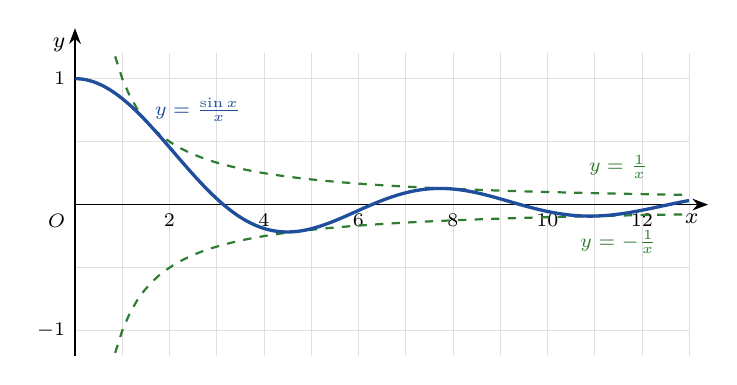
\begin{tikzpicture}[x=0.6cm,y=1.6cm,font=\footnotesize]
\draw[gray!25,very thin] (0,-1.2) grid[xstep=1,ystep=0.5] (13,1.2);
\draw[-{Stealth[length=2mm]}] (0,0)--(13.4,0) node[below left]{$x$};
\draw[-{Stealth[length=2mm]}] (0,-1.2)--(0,1.4) node[below left]{$y$};
\foreach \t in {2,4,6,8,10,12} \node[below,font=\scriptsize] at (\t,0){$\t$};
\foreach \t in {-1,1} \node[left,font=\scriptsize] at (0,\t){$\t$};
\node[below left,font=\scriptsize] at (0,0){$O$};
\draw[cRem,thick,dashed,domain=0.85:13,samples=80] plot(\x,{1/\x});
\draw[cRem,thick,dashed,domain=0.85:13,samples=80] plot(\x,{-1/\x});
\draw[cDef,very thick,domain=0.01:13,samples=200] plot(\x,{sin(\x r)/\x});
\node[cDef,font=\scriptsize] at (2.6,0.75){$y=\frac{\sin x}{x}$};
\node[cRem,font=\scriptsize] at (11.5,0.3){$y=\frac1x$};
\node[cRem,font=\scriptsize] at (11.5,-0.3){$y=-\frac1x$};
\end{tikzpicture}\end{LTR}\end{center}
\end{mithal}
%================================================================
\section{السلوك التقاربي -- المستقيمات المقاربة}
\begin{khassia}[التفسير الهندسي للنهايات]
\begin{itemize}
\item \bx{\Lim{x\to a^{\pm}}f(x)=\pm\infty}: المستقيم ذو المعادلة \bx{x=a} \textbf{مقارب عمودي} لـ $(C_f)$.
\item \bx{\Lim{x\to\pm\infty}f(x)=b}: المستقيم ذو المعادلة \bx{y=b} \textbf{مقارب أفقي} لـ $(C_f)$ بجوار $\pm\infty$.
\item \bx{\Lim{x\to\pm\infty}\big[f(x)-(ax+b)\big]=0} \ ($a\neq0$): المستقيم ذو المعادلة \bx{y=ax+b} \textbf{مقارب مائل} لـ $(C_f)$ بجوار $\pm\infty$.\par
بصفة مكافئة: إذا كتبنا $f(x)=ax+b+\theta(x)$ مع $\Lim{x\to\pm\infty}\theta(x)=0$.
\item \bx{\Lim{x\to\pm\infty}\big[f(x)-g(x)\big]=0}: المنحنيان $(C_f)$ و $(C_g)$ \textbf{متقاربان} بجوار $\pm\infty$.
\end{itemize}
\end{khassia}

\begin{khassia}[الوضع النسبي لـ $(C_f)$ و $(\Delta):y=ax+b$]
ندرس إشارة الفرق $d(x)=f(x)-(ax+b)$:
\begin{itemize}
\item $d(x)>0$: $(C_f)$ يقع \textbf{فوق} $(\Delta)$ ؛ \quad $d(x)<0$: $(C_f)$ يقع \textbf{تحت} $(\Delta)$ ؛
\item $d(x_0)=0$: $(C_f)$ يقطع $(\Delta)$ في النقطة $A\big(x_0;f(x_0)\big)$.
\end{itemize}
(نفس الطريقة مع مقارب أفقي $y=b$ أو منحنٍ $(C_g)$.)
\end{khassia}

\begin{mithal}[مقارب أفقي ومقارب عمودي: $f(x)=\dfrac{2x+1}{x-1}$]
\RL{0.56}{
\textbf{عند $\pm\infty$:} $\Lim{x\to\pm\infty}\dfrac{2x+1}{x-1}=\Lim{x\to\pm\infty}\dfrac{2x}{x}=2$\par
إذن \bx{y=2} مقارب أفقي بجوار $\pm\infty$.\par\smallskip
\textbf{عند $1$:} البسط يؤول إلى $3$، والمقام إلى $0^{+}$ من اليمين و $0^{-}$ من اليسار:\par
$\Lim{x\to1^{+}}f(x)=+\infty$ ، \ $\Lim{x\to1^{-}}f(x)=-\infty$\par
إذن \bx{x=1} مقارب عمودي.\par\smallskip
\textbf{الوضع النسبي:} $f(x)-2=\dfrac{3}{x-1}$\par
على $]1;+\infty[$: $(C_f)$ فوق $y=2$؛ \ على $]-\infty;1[$: تحته.
}{0.4}{
\begin{GR}{-3}{5}{-3}{7}{0.46}
\Ticks{-2,2,4}{-2,2,4,6}
\draw[cRem,thick,dashed] (-3,2)--(5,2);
\draw[cRem,thick,dashed] (1,-3)--(1,7);
\draw[cDef,very thick,domain=-3:0.4,samples=60] plot(\x,{(2*\x+1)/(\x-1)});
\draw[cDef,very thick,domain=1.6:5,samples=60] plot(\x,{(2*\x+1)/(\x-1)});
\node[cRem,font=\scriptsize] at (-2.2,2.5){$y=2$};
\node[cRem,font=\scriptsize] at (1.8,6.3){$x=1$};
\end{GR}
}
\end{mithal}

\begin{mithal}[مقارب مائل: $f(x)=\dfrac{x^{2}+x+1}{x-1}$ على $\R-\{1\}$]
بالقسمة: $x^{2}+x+1=(x-1)(x+2)+3$، إذن \bx{f(x)=x+2+\dfrac{3}{x-1}}.
\begin{itemize}
\item $\Lim{x\to\pm\infty}\big[f(x)-(x+2)\big]=\Lim{x\to\pm\infty}\dfrac{3}{x-1}=0$: \ \bx{y=x+2} مقارب مائل بجوار $\pm\infty$.
\item $\Lim{x\to1^{+}}f(x)=+\infty$ و $\Lim{x\to1^{-}}f(x)=-\infty$: \ \bx{x=1} مقارب عمودي.
\item إشارة $\dfrac{3}{x-1}$: \ $(C_f)$ تحت $(\Delta)$ على $]-\infty;1[$ ، وفوقه على $]1;+\infty[$.
\end{itemize}
\begin{TAB}
\tkzTabInit[lgt=3.2,espcl=3.6]{$x$/1,$f(x)-(x+2)$/1,\hbox{\ar{الوضع النسبي}}/1}{$-\infty$,$1$,$+\infty$}
\tkzTabLine{,-,d,+,}
\tkzTabLine{,\mbox{\ar{$(C_f)$ تحت $(\Delta)$}},d,\mbox{\ar{$(C_f)$ فوق $(\Delta)$}},}
\end{TAB}
\begin{GR}{-4}{6}{-5}{11}{0.42}
\Ticks{-2,2,4}{-4,-2,2,4,6,8,10}
\draw[cRem,thick,dashed,domain=-4:6] plot(\x,{\x+2});
\draw[cRem,thick,dashed] (1,-5)--(1,11);
\draw[cDef,very thick,domain=-4:0.6,samples=80] plot(\x,{\x+2+3/(\x-1)});
\draw[cDef,very thick,domain=1.39:6,samples=80] plot(\x,{\x+2+3/(\x-1)});
\fill (1,3) circle (2pt) node[left,font=\scriptsize]{$\Omega$};
\node[cRem,font=\scriptsize] at (4.4,8.4){$(\Delta):y=x+2$};
\node[cDef,font=\scriptsize] at (2.6,10){$(C_f)$};
\end{GR}
\end{mithal}

\begin{khassia}[تعيين المقارب المائل -- رياضيات وتقني رياضي]
إذا كان \ $\Lim{x\to\pm\infty}\dfrac{f(x)}{x}=a$ \ ($a\neq0$) \ و \ $\Lim{x\to\pm\infty}\big[f(x)-ax\big]=b$ \ (عدد حقيقي) فإن المستقيم ذا المعادلة \bx{y=ax+b} مقارب مائل لـ $(C_f)$ بجوار $\pm\infty$.
\end{khassia}
\begin{mithal}[$f(x)=\sqrt{x^{2}+1}$ بجوار $+\infty$]
من أجل $x>0$:
\[ \frac{f(x)}{x}=\sqrt{1+\frac{1}{x^{2}}}\ \xrightarrow[x\to+\infty]{}\ 1=a \qquad\qquad f(x)-x=\frac{1}{\sqrt{x^{2}+1}+x}\ \xrightarrow[x\to+\infty]{}\ 0=b \]
إذن \bx{y=x} مقارب مائل بجوار $+\infty$، و $f(x)-x>0$: $(C_f)$ فوق المقارب.
\end{mithal}

\begin{mithal}[منحنيان متقاربان: $f(x)=x^{2}+\dfrac1x$]
\[ \Lim{x\to\pm\infty}\left[f(x)-x^{2}\right]=\Lim{x\to\pm\infty}\frac1x=0 \]
إذن $(C_f)$ والقطع المكافئ $(P):y=x^{2}$ \bxt{متقاربان بجوار $\pm\infty$}.\par
$(C_f)$ فوق $(P)$ على $]0;+\infty[$، وتحته على $]-\infty;0[$.
\end{mithal}

\begin{mithal}[قراءة النهايات من التمثيل البياني]
\RL{0.48}{
$(C_f)$ تمثيل الدالة $f$ المعرفة على $\R-\{-2;2\}$ بـ:
\[ f(x)=\frac{2x^{2}}{x^{2}-4} \]
نقرأ من الشكل:\par
$\Lim{x\to-\infty}f(x)=\Lim{x\to+\infty}f(x)=2$ ؛\par
$\Lim{x\to-2^{-}}f(x)=+\infty$ ، $\Lim{x\to-2^{+}}f(x)=-\infty$ ؛\par
$\Lim{x\to2^{-}}f(x)=-\infty$ ، $\Lim{x\to2^{+}}f(x)=+\infty$.\par
المقاربات: $y=2$ ، $x=-2$ ، $x=2$ (والمنحنى متناظر بالنسبة إلى محور التراتيب: $f$ زوجية).
}{0.48}{
\begin{GR}{-6}{6}{-5}{7}{0.36}
\Ticks{-4,-2,2,4}{-4,-2,2,4,6}
\draw[cRem,thick,dashed] (-6,2)--(6,2);
\draw[cRem,thick,dashed] (-2,-5)--(-2,7);
\draw[cRem,thick,dashed] (2,-5)--(2,7);
\draw[cDef,very thick,domain=-6:-2.37,samples=60] plot(\x,{2*\x*\x/(\x*\x-4)});
\draw[cDef,very thick,domain=2.37:6,samples=60] plot(\x,{2*\x*\x/(\x*\x-4)});
\draw[cDef,very thick,domain=-1.69:1.69,samples=80] plot(\x,{2*\x*\x/(\x*\x-4)});
\end{GR}
}
\end{mithal}

%================================================================
\section{الاستمرارية}
\begin{tarif}
$f$ دالة معرفة على مجال $I$ و $a\in I$.
\begin{itemize}
\item $f$ \textbf{مستمرة عند $a$} معناه \bx{\Lim{x\to a}f(x)=f(a)}.
\item $f$ \textbf{مستمرة على $I$} إذا كانت مستمرة عند كل عدد من $I$. \ بيانيًا: \textbf{نرسم منحناها على $I$ دون رفع القلم}.
\end{itemize}
\end{tarif}

\begin{khassia}[الدوال المألوفة]
\begin{itemize}
\item الدوال كثيرات الحدود، $\sin$ و $\cos$ مستمرة على $\R$؛ الدالة $x\mapsto|x|$ مستمرة على $\R$.
\item الدوال الناطقة مستمرة على كل مجال من مجموعة تعريفها؛ الدالة $x\mapsto\sqrt{x}$ مستمرة على $[0;+\infty[$.
\item كل دالة ناتجة عن عمليات (مجموع، جداء، حاصل قسمة، تركيب) على دوال مستمرة هي مستمرة على كل مجال من مجموعة تعريفها.
\end{itemize}
\end{khassia}

\begin{mithal}[استمرار دالة معرفة بجزأين]
\RL{0.6}{
$f(x)=\begin{cases}x+1 & x<1\\ -x+4 & x\geqslant1\end{cases}$\par
$f(1)=3$ و $\Lim{x\to1^{+}}f(x)=3$\par
لكن $\Lim{x\to1^{-}}f(x)=2\neq f(1)$.\par
إذن \bxt{$f$ غير مستمرة عند $1$}: نرفع القلم عند $x=1$.\par\smallskip
\textbf{مع وسيط:} $g(x)=\begin{cases}x^{2}+ax & x\leqslant1\\ 2x+3 & x>1\end{cases}$\par
$g(1)=1+a$ و $\Lim{x\to1^{+}}g(x)=5$.\par
$g$ مستمرة عند $1$ معناه $1+a=5$، أي \bx{a=4}.
}{0.4}{
\begin{GR}{-1}{4}{-0.5}{4}{0.62}
\Ticks{1,2,3}{1,2,3}
\draw[cDef,very thick] (-1,0)--(1,2);
\draw[cDef,very thick] (1,3)--(4,0);
\draw[cDef,thick,fill=white] (1,2) circle (2.4pt);
\fill[cDef] (1,3) circle (2.4pt);
\draw[dotted] (1,0)--(1,3)--(0,3);
\end{GR}
}
\end{mithal}

\begin{molahada}[الاستمرار في جدول التغيرات]
\textbf{اصطلاحًا:} الأسهم المائلة في جدول التغيرات تعني أن الدالة \textbf{مستمرة ورتيبة تمامًا} على المجال الموافق. الخط المزدوج $\|$ يعني أن الدالة غير معرفة عند تلك القيمة.
\end{molahada}

\subsection{مبرهنة القيم المتوسطة}
\begin{khassia}[مبرهنة القيم المتوسطة]
إذا كانت $f$ \textbf{مستمرة} على مجال $[a;b]$، فإنه من أجل كل عدد حقيقي $k$ محصور بين $f(a)$ و $f(b)$ توجد \textbf{على الأقل} قيمة $c$ من $[a;b]$ حيث \bx{f(c)=k}.
\end{khassia}
\begin{khassia}[النتيجة (الحالة الخاصة) -- وجود ووحدانية الحل]
إذا كانت $f$ \textbf{مستمرة} و\textbf{رتيبة تمامًا} على $[a;b]$ و \bx{f(a)\times f(b)<0} فإن المعادلة $f(x)=0$ تقبل \textbf{حلًا وحيدًا} $\alpha$ في $]a;b[$.\par
تبقى صحيحة على مجال مفتوح أو غير محدود باستعمال النهايات بدل الصور.
\end{khassia}

\begin{mithal}[$f(x)=x^{3}-3x+1$]
\RL{0.6}{
$f$ مستمرة على $\R$ (كثير حدود)، و:\par
$f(-2)=-1$ ، $f(-1)=3$ ، $f(0)=1$ ، $f(1)=-1$ ، $f(2)=3$.\par
حسب مبرهنة القيم المتوسطة، تقبل المعادلة $f(x)=0$ حلًا على الأقل في كل من المجالات $]-2;-1[$ ، $]0;1[$ ، $]1;2[$.\par
$f'(x)=3x^{2}-3$: $f$ رتيبة تمامًا على كل من $]-\infty;-1]$ ، $[-1;1]$ ، $[1;+\infty[$، إذن للمعادلة \bxt{ثلاثة حلول بالضبط}.
}{0.36}{
\begin{GR}{-2.5}{2.5}{-2}{4}{0.62}
\Ticks{-2,-1,1,2}{-1,1,2,3}
\draw[cDef,very thick,domain=-2.3:2.3,samples=100] plot(\x,{\x*\x*\x-3*\x+1});
\fill[cThm] (-1.879,0) circle (1.8pt);
\fill[cThm] (0.347,0) circle (1.8pt);
\fill[cThm] (1.532,0) circle (1.8pt);
\end{GR}
}
\end{mithal}

\subsection{حصر الحل $\alpha$: التنصيف والمسح}
\begin{tariqa}[طريقة التنصيف]
نعلم أن $\alpha\in]a;b[$. نحسب $m=\dfrac{a+b}{2}$ و $f(m)$:
\begin{itemize}
\item إذا كان $f(a)\times f(m)<0$ فإن $\alpha\in]a;m[$ ؛ \quad وإذا كان $f(m)\times f(b)<0$ فإن $\alpha\in]m;b[$.
\item نكرر بالمجال الجديد حتى نحصل على السعة المطلوبة.
\end{itemize}
\end{tariqa}
\begin{tariqa}[طريقة المسح (الجدولة)]
نقسم $[a;b]$ إلى مجالات طولها $h$ (مثلًا $0{,}1$ ثم $0{,}01$) ونحسب الصور بالحاسبة؛ $\alpha$ يقع في المجال الذي تتغير فيه إشارة $f$.\par
مثال: الحل الواقع في $]0;1[$ من المثال السابق، بخطوة $0{,}1$:
\[ f(0{,}3)=0{,}127>0 \qquad\qquad f(0{,}4)=-0{,}136<0 \]
إذن \bx{0{,}3<\alpha<0{,}4}.
\end{tariqa}

\begin{mithal}[{$f(x)=\dfrac{1}{x-1}-\sqrt{x}$ على $]1;+\infty[$}]
\begin{itemize}
\item $f'(x)=-\dfrac{1}{(x-1)^{2}}-\dfrac{1}{2\sqrt{x}}<0$: $f$ مستمرة ومتناقصة تمامًا على $]1;+\infty[$.
\item $f(1{,}1)\approx8{,}95>0$ و $f(2{,}3)\approx-0{,}75<0$، إذن المعادلة $f(x)=0$ تقبل حلًا وحيدًا $\alpha\in]1{,}1;2{,}3[$.
\item التنصيف (نحتفظ بالنصف الذي تتغير فيه الإشارة):\par
$m=1{,}7$: \ $f(1{,}7)\approx0{,}12>0$، إذن $\alpha\in]1{,}7;2{,}3[$.\par
$m=2$: \ $f(2)\approx-0{,}41<0$، إذن $\alpha\in]1{,}7;2[$.\par
$m=1{,}85$: \ $f(1{,}85)\approx-0{,}18<0$، إذن \bx{1{,}7<\alpha<1{,}85} \ (سعة $0{,}15$).
\item $f(\alpha)=0\iff\dfrac{1}{\alpha-1}=\sqrt{\alpha}$، وبالتربيع: $\alpha(\alpha-1)^{2}=1$، أي \bx{\alpha^{3}-2\alpha^{2}+\alpha-1=0}.
\end{itemize}
\end{mithal}

\subsection{صورة مجال بدالة مستمرة ورتيبة تمامًا}
\begin{khassia}
$f$ مستمرة ورتيبة تمامًا على $[a;b]$:
\begin{itemize}
\item إذا كانت متزايدة تمامًا: \bx{f([a;b])=[f(a);f(b)]} ؛ \quad إذا كانت متناقصة تمامًا: \bx{f([a;b])=[f(b);f(a)]}.
\item على مجال مفتوح أو غير محدود نستعمل النهايات؛ مثلًا إذا كانت $f$ متزايدة تمامًا على $]a;+\infty[$:
\[ f\big(]a;+\infty[\big)=\left]\Lim{x\to a^{+}}f(x)\,;\,\Lim{x\to+\infty}f(x)\right[ \]
\end{itemize}
\end{khassia}
\begin{mithal}
$f(x)=x^{3}-3x+1$:
\begin{itemize}
\item $f$ متناقصة تمامًا على $[-1;1]$، إذن $f([-1;1])=[f(1);f(-1)]=\bx{[-1;3]}$.
\item $f$ متزايدة تمامًا على $]1;+\infty[$، إذن $f(]1;+\infty[)=\bx{]-1;+\infty[}$.
\end{itemize}
\end{mithal}
%================================================================
\section{الاشتقاقية}
\subsection{العدد المشتق والمماس}
\begin{tarif}
$f$ دالة معرفة على مجال مفتوح يشمل $x_0$. نقول إن $f$ \textbf{قابلة للاشتقاق عند $x_0$} إذا كان:
\[ \Lim{x\to x_0}\frac{f(x)-f(x_0)}{x-x_0}=\ell \qquad(\ell\in\R), \]
أو بوضع $x=x_0+h$: \ $\Lim{h\to0}\dfrac{f(x_0+h)-f(x_0)}{h}=\ell$.\par
العدد $\ell$ يسمى \textbf{العدد المشتق} للدالة $f$ عند $x_0$ ونكتب \bx{f'(x_0)=\ell}.
\end{tarif}

\begin{khassia}[التفسير الهندسي ومعادلة المماس]
$f'(x_0)$ هو \textbf{معامل توجيه المماس} $(T)$ للمنحنى $(C_f)$ في النقطة $A\big(x_0;f(x_0)\big)$، ومعادلته:
\[ \bx{(T):\ y=f'(x_0)(x-x_0)+f(x_0)} \]
\begin{itemize}
\item $f'(x_0)=0$: المماس \textbf{يوازي محور الفواصل} ($y=f(x_0)$).
\item قراءة $f'(x_0)$ بيانيًا: نختار نقطتين $A(x_A;y_A)$ و $B(x_B;y_B)$ من المماس، فيكون $f'(x_0)=\dfrac{y_B-y_A}{x_B-x_A}$.
\end{itemize}
\end{khassia}

\begin{mithal}[أسئلة المماس: $f(x)=\dfrac{3x-4}{x-2}$ على $\R-\{2\}$]
$f'(x)=\dfrac{3(x-2)-(3x-4)}{(x-2)^{2}}=\bx{\dfrac{-2}{(x-2)^{2}}}$.
\begin{itemize}
\item \textbf{المماس عند النقطة ذات الفاصلة $1$:} \ $f(1)=1$ و $f'(1)=-2$:
\[ (T):\ y=-2(x-1)+1 \quad\Longrightarrow\quad \bx{y=-2x+3} \]
\item \textbf{مماسات معامل توجيهها $-2$:} نحل $f'(x)=-2$:
\[ \frac{-2}{(x-2)^{2}}=-2\iff(x-2)^{2}=1\iff \bx{x\in\{1;3\}} \]
\item \textbf{مماسات توازي المستقيم $y=-\frac12x-1$:} نحل $f'(x)=-\frac12$:
\[ (x-2)^{2}=4\iff \bx{x\in\{0;4\}} \]
\item \textbf{مماسات تعامد المستقيم $y=8x$:} نحل $8f'(x)=-1$:
\[ (x-2)^{2}=16\iff \bx{x\in\{-2;6\}} \]
\item \textbf{مماس يشمل النقطة $B(2;2)$:} نحل $2=f'(x_0)(2-x_0)+f(x_0)$ ($x_0\neq2$):
\[ \frac{2}{x_0-2}+\frac{3x_0-4}{x_0-2}=2\iff\frac{x_0+2}{x_0-2}=0\iff\bx{x_0=-2} \]
\item \textbf{المماس عند النقطة ذات الترتيب $5$:} نحل $f(x_0)=5$:
\[ 3x_0-4=5x_0-10\iff x_0=3 \qquad (T):\ y=-2(x-3)+5 \quad\Longrightarrow\quad \bx{y=-2x+11} \]
\end{itemize}
\end{mithal}

\subsection{الاشتقاق من اليمين ومن اليسار -- نصف المماس}
\begin{khassia}
\begin{itemize}
\item إذا كان $\Lim{x\to x_0^{+}}\dfrac{f(x)-f(x_0)}{x-x_0}=a$ (عدد حقيقي): $f$ قابلة للاشتقاق \textbf{على يمين} $x_0$، و $f'_d(x_0)=a$؛ يقبل $(C_f)$ عند $A$ \textbf{نصف مماس} معامل توجيهه $a$.
\item إذا كان $\Lim{x\to x_0^{-}}\dfrac{f(x)-f(x_0)}{x-x_0}=b$: $f$ قابلة للاشتقاق \textbf{على يسار} $x_0$، و $f'_g(x_0)=b$.
\item $f$ قابلة للاشتقاق عند $x_0$ $\iff$ \bx{f'_d(x_0)=f'_g(x_0)}.
\item إذا كان $f'_d(x_0)\neq f'_g(x_0)$: $f$ غير قابلة للاشتقاق عند $x_0$، و $A$ \textbf{نقطة زاوية} (نصفا مماسين مختلفين).
\item إذا كانت النهاية $+\infty$ أو $-\infty$: $f$ غير قابلة للاشتقاق، و $(C_f)$ يقبل عند $A$ \textbf{نصف مماس عمودي} معادلته $x=x_0$ (موجّه نحو الأعلى أو نحو الأسفل حسب الإشارة وجهة الاقتراب).
\end{itemize}
\end{khassia}

\begin{mithal}[نقطة زاوية ونصف مماس عمودي]
\textbf{1.} $f(x)=|x^{2}-4|$ عند $2$ ($f(2)=0$):\par
من أجل $x>2$: \quad $\dfrac{f(x)-f(2)}{x-2}=\dfrac{x^{2}-4}{x-2}=x+2\ \longrightarrow\ 4$\par
من أجل $-2<x<2$: \quad $\dfrac{f(x)-f(2)}{x-2}=\dfrac{-\left(x^{2}-4\right)}{x-2}=-(x+2)\ \longrightarrow\ -4$\par
$f'_d(2)=4$ و $f'_g(2)=-4$ مختلفان: \bxt{$A(2;0)$ نقطة زاوية}.\par\smallskip
\textbf{2.} $g(x)=\sqrt{x}$ عند $0$: \quad $\dfrac{g(x)-g(0)}{x-0}=\dfrac{1}{\sqrt{x}}\ \longrightarrow\ +\infty$\par
$g$ غير قابلة للاشتقاق عند $0$، و $(C_g)$ يقبل \bxt{نصف مماس عمودي} عند $O$.

\begin{GR}{-3}{3}{-0.5}{5}{0.58}
\Ticks{-2,-1,1,2}{1,2,3,4}
\draw[cDef,very thick,domain=-2.9:2.9,samples=120] plot(\x,{abs(\x*\x-4)});
\draw[cThm,thick,-{Stealth}] (2,0)--(2.45,1.8);
\draw[cThm,thick,-{Stealth}] (2,0)--(1.55,1.8);
\fill (2,0) circle (1.8pt) node[below,font=\scriptsize]{$A$};
\end{GR}

\end{mithal}

\begin{khassia}[الاستمرارية والاشتقاقية]
إذا كانت $f$ قابلة للاشتقاق عند $x_0$ فإنها \textbf{مستمرة} عند $x_0$. \ \textbf{العكس غير صحيح}: $x\mapsto|x|$ مستمرة عند $0$ وغير قابلة للاشتقاق عنده ($f'_d(0)=1$ ، $f'_g(0)=-1$).
\end{khassia}

\subsection{التقريب التآلفي}
\begin{khassia}
إذا كانت $f$ قابلة للاشتقاق عند $x_0$ فإنه من أجل $h$ قريب من $0$: \quad \bx{f(x_0+h)\approx f(x_0)+h\,f'(x_0)}\par
(نستبدل المنحنى بمماسه بجوار $x_0$).
\end{khassia}
\begin{mithal}
\begin{itemize}
\item $f(x)=\sqrt{x}$ ، $x_0=4$ ، $h=0{,}02$ ، $f'(4)=\dfrac{1}{2\sqrt4}=\dfrac14$:
\[ \sqrt{4{,}02}\approx2+0{,}02\times\frac14=\bx{2{,}005} \]
(القيمة بالحاسبة: $2{,}00499\ldots$).
\item بجوار $0$: $(1+h)^{n}\approx1+nh$ ، $\sqrt{1+h}\approx1+\dfrac h2$ ، $\sin h\approx h$ ، $\cos h\approx1$.
\end{itemize}
\end{mithal}

\subsection{مشتقات الدوال المألوفة والعمليات}
\begin{khassia}[مشتقات الدوال المألوفة]
\begin{center}\renewcommand{\arraystretch}{1.9}
\begin{tabular}{|C|c|C|}\hline
\rowcolor{cSec!12} مجال قابلية الاشتقاق & $f'(x)$ & $f(x)$\\\hline
$\R$ & $0$ & $c$ (ثابت)\\\hline
$\R$ & $a$ & $ax+b$\\\hline
$\R$ & $nx^{n-1}$ & $x^{n}$ \ ($n\in\N^{*}$)\\\hline
$\R^{*}$ & $-\dfrac{1}{x^{2}}$ & $\dfrac1x$\\\hline
$\R^{*}$ & $-\dfrac{n}{x^{n+1}}$ & $\dfrac{1}{x^{n}}$\\\hline
$]0;+\infty[$ & $\dfrac{1}{2\sqrt{x}}$ & $\sqrt{x}$\\\hline
$\R$ & $\cos x$ & $\sin x$\\\hline
$\R$ & $-\sin x$ & $\cos x$\\\hline
\end{tabular}\end{center}
\end{khassia}

\begin{khassia}[العمليات على الدوال المشتقة]
$u$ و $v$ قابلتان للاشتقاق على مجال $I$ ، $k$ عدد حقيقي، $n\in\N^{*}$:
\begin{align*}
(u+v)'&=u'+v' & (ku)'&=ku' & (uv)'&=u'v+uv'\\
\left(\frac1v\right)'&=-\frac{v'}{v^{2}} & \left(\frac uv\right)'&=\frac{u'v-uv'}{v^{2}} & \left(u^{n}\right)'&=nu'u^{n-1}\\
\left(\frac{1}{u^{n}}\right)'&=-\frac{nu'}{u^{n+1}} & \left(\sqrt{u}\right)'&=\frac{u'}{2\sqrt{u}}\ (u>0) & \big(v\circ u\big)'&=u'\times\left(v'\circ u\right)\\
\big(\sin(ax+b)\big)'&=a\cos(ax+b) & \big(\cos(ax+b)\big)'&=-a\sin(ax+b) & \big(f(ax+b)\big)'&=af'(ax+b)
\end{align*}
($v\ne0$ على $I$ في قواعد القسمة، و $u\neq0$ في $\frac{1}{u^{n}}$.)
\end{khassia}

\begin{mithal}
\begin{itemize}
\item $f(x)=\left(x^{4}+2x\right)^{6}$: \ $f'(x)=6\left(4x^{3}+2\right)\left(x^{4}+2x\right)^{5}$.
\item $f(x)=\left(\dfrac{3x-1}{2x-4}\right)^{2}=u^{2}$ مع $u(x)=\dfrac{3x-1}{2x-4}$:
\[ u'(x)=\frac{3(2x-4)-2(3x-1)}{(2x-4)^{2}}=\frac{-10}{(2x-4)^{2}}\qquad f'(x)=2u'u=\frac{-20(3x-1)}{(2x-4)^{3}} \]
\item $f(x)=\dfrac{1}{\left(x^{2}+3\right)^{3}}$: \ $f'(x)=-\dfrac{3\times2x}{\left(x^{2}+3\right)^{4}}=-\dfrac{6x}{\left(x^{2}+3\right)^{4}}$.
\item $f(x)=\sqrt{x^{2}-2x+5}$ \ (لدينا $x^{2}-2x+5>0$ لأن $\Delta=-16<0$):
\[ f'(x)=\frac{2x-2}{2\sqrt{x^{2}-2x+5}}=\frac{x-1}{\sqrt{x^{2}-2x+5}} \]
\item $f(x)=\sin\left(2x-\frac{\pi}{3}\right)$: \ $f'(x)=2\cos\left(2x-\frac{\pi}{3}\right)$ ؛ \quad $g(x)=\cos^{2}x$: \ $g'(x)=-2\sin x\cos x$.
\item \textbf{المشتقات المتتابعة:} $f(x)=x^{4}-2x^{3}+x-1$:
\[ f'(x)=4x^{3}-6x^{2}+1\qquad f''(x)=12x^{2}-12x\qquad f^{(3)}(x)=24x-12\qquad f^{(4)}(x)=24 \]
\end{itemize}
\end{mithal}

\subsection{المشتقات المتتابعة}
\begin{tarif}
$f$ قابلة للاشتقاق على مجال $I$ ومشتقتها $f'$. إذا كانت $f'$ قابلة للاشتقاق على $I$ فإن مشتقتها تسمى \textbf{المشتقة الثانية} لـ $f$ ونرمز لها بـ \bx{f''=(f')'}.\par
وبنفس الطريقة نعرّف المشتقة الثالثة $f^{(3)}=(f'')'$، ثم المشتقة من الرتبة $n$: \bx{f^{(n)}=\left(f^{(n-1)}\right)'} \ ($n\in\N^{*}$، مع $f^{(0)}=f$).
\end{tarif}
\begin{mithal}
\begin{itemize}
\item $f(x)=\dfrac1x$ على $\R^{*}$:
\[ f'(x)=-\frac{1}{x^{2}}\qquad f''(x)=\frac{2}{x^{3}}\qquad f^{(3)}(x)=-\frac{6}{x^{4}}\qquad f^{(4)}(x)=\frac{24}{x^{5}} \]
\item $g(x)=\sin2x$ على $\R$:
\[ g'(x)=2\cos2x\qquad g''(x)=-4\sin2x\qquad g^{(3)}(x)=-8\cos2x\qquad g^{(4)}(x)=16\sin2x \]
نلاحظ أن \bx{g''(x)=-4g(x)} و $g^{(4)}=16g$.
\item كثير حدود من الدرجة $n$: مشتقته من الرتبة $n$ ثابتة، ومشتقاته من رتبة أكبر من $n$ معدومة.
\end{itemize}
\end{mithal}
\begin{molahada}
تستعمل المشتقة الثانية في دراسة \textbf{نقطة الانعطاف} (إشارة $f''$)، وفي دراسة إشارة $f'$ عندما يصعب حل $f'(x)=0$ (اتجاه تغير $f'$).
\end{molahada}

%================================================================
\section{الدوال المثلثية $x\mapsto\cos(\omega x+\varphi)$ و $x\mapsto\sin(\omega x+\varphi)$}
\subsection{الدالتان $\sin$ و $\cos$}
\begin{khassia}
\begin{itemize}
\item $\sin$ و $\cos$ معرفتان وقابلتان للاشتقاق على $\R$، و \bx{\sin'=\cos} ، \bx{\cos'=-\sin}.
\item \textbf{دوريتان} دورهما $2\pi$: $\sin(x+2\pi)=\sin x$ و $\cos(x+2\pi)=\cos x$.
\item $\sin$ \textbf{فردية} (منحناها متناظر بالنسبة إلى $O$) و $\cos$ \textbf{زوجية} (منحناها متناظر بالنسبة إلى محور التراتيب).
\item من أجل كل $x$: $-1\leqslant\sin x\leqslant1$ و $-1\leqslant\cos x\leqslant1$.
\end{itemize}
\end{khassia}
\begin{mithal}[تغيرات $\cos$ على $[0;\pi]$ و $\sin$ على $\left[-\frac{\pi}{2};\frac{\pi}{2}\right]$]
\RL{0.48}{
\begin{TAB}
\tkzTabInit[lgt=1.5,espcl=2.2]{$x$/1,$\sin'(x)$/1,$\sin x$/1.6}{$-\frac{\pi}{2}$,$\frac{\pi}{2}$}
\tkzTabLine{,+,}
\tkzTabVar{-/$-1$,+/$1$}
\end{TAB}
}{0.48}{
\begin{TAB}
\tkzTabInit[lgt=1.5,espcl=2.2]{$x$/1,$\cos'(x)$/1,$\cos x$/1.6}{$0$,$\pi$}
\tkzTabLine{,-,}
\tkzTabVar{+/$1$,-/$-1$}
\end{TAB}
}
\begin{GR}{-6.6}{6.6}{-1.6}{1.6}{0.75}
\foreach \t/\l in {-6.2832/-2\pi,-3.1416/-\pi,3.1416/\pi,6.2832/2\pi}{\node[below,font=\scriptsize] at (\t,0){$\l$};}
\node[left,font=\scriptsize] at (0,1){$1$}; \node[left,font=\scriptsize] at (0,-1){$-1$};
\draw[cDef,very thick,domain=-6.6:6.6,samples=200] plot(\x,{sin(\x r)});
\draw[cThm,very thick,dashed,domain=-6.6:6.6,samples=200] plot(\x,{cos(\x r)});
\node[cDef] at (2.2,1.3){$y=\sin x$};
\node[cThm] at (-4.2,1.3){$y=\cos x$};
\end{GR}
\end{mithal}

\subsection{الدالتان $x\mapsto\cos(\omega x+\varphi)$ و $x\mapsto\sin(\omega x+\varphi)$}
\begin{khassia}
$\omega$ و $\varphi$ عددان حقيقيان مع $\omega\neq0$. الدالتان $f(x)=\cos(\omega x+\varphi)$ و $g(x)=\sin(\omega x+\varphi)$ قابلتان للاشتقاق على $\R$ (مركب دالة تآلفية ودالة مثلثية) و:
\[ \bx{f'(x)=-\omega\sin(\omega x+\varphi)} \qquad\qquad \bx{g'(x)=\omega\cos(\omega x+\varphi)} \]
\begin{itemize}
\item هما \textbf{دوريتان} ودورهما \bx{T=\dfrac{2\pi}{|\omega|}} لأن $\omega(x+T)+\varphi=\omega x+\varphi\pm2\pi$.
\item يكفي دراستهما على \textbf{مجال طوله $T$}، ثم نكمل المنحنى بانسحابات شعاعها $kT\,\vec{i}$ ($k\in\Z$).
\item المشتقة الثانية: $f''=-\omega^{2}f$ و $g''=-\omega^{2}g$، أي \bx{f''+\omega^{2}f=0}.
\end{itemize}
\end{khassia}
\begin{tariqa}[دراسة $x\mapsto A\cos(\omega x+\varphi)$ أو $x\mapsto A\sin(\omega x+\varphi)$]
\begin{enumerate}
\item نعيّن الدور $T=\frac{2\pi}{|\omega|}$ ونختار مجالًا طوله $T$.
\item نحسب $f'(x)$، ونحل $f'(x)=0$ في هذا المجال (معادلة مثلثية أساسية).
\item ندرس إشارة $f'(x)$ بوضع $X=\omega x+\varphi$ (موقع $X$ على الدائرة المثلثية)، ونشكل جدول التغيرات.
\item نرسم المنحنى على المجال، ونكمله بالانسحاب.
\end{enumerate}
\end{tariqa}
\begin{mithal}[{دراسة $f(x)=2\cos\left(2x-\frac{\pi}{3}\right)$}]
\begin{itemize}
\item \textbf{الدور:} $T=\dfrac{2\pi}{2}=\bx{\pi}$؛ ندرس $f$ على $[0;\pi]$.
\item \textbf{المشتقة:} $f'(x)=2\times\left(-2\sin\left(2x-\frac{\pi}{3}\right)\right)=\bx{-4\sin\left(2x-\frac{\pi}{3}\right)}$.
\item نضع $X=2x-\frac{\pi}{3}$: لما $x\in[0;\pi]$ يكون $X\in\left[-\frac{\pi}{3};\frac{5\pi}{3}\right]$.\par
$\sin X=0\iff X\in\{0;\pi\}\iff x\in\left\{\frac{\pi}{6};\frac{2\pi}{3}\right\}$؛\ \ $\sin X<0$ لما $X\in\left[-\frac{\pi}{3};0\right[$ أو $X\in\left]\pi;\frac{5\pi}{3}\right]$، و $\sin X>0$ لما $X\in]0;\pi[$.
\item الصور: $f(0)=2\cos\left(-\frac{\pi}{3}\right)=1$ ، $f\left(\frac{\pi}{6}\right)=2\cos0=2$ ، $f\left(\frac{2\pi}{3}\right)=2\cos\pi=-2$ ، $f(\pi)=1$.
\end{itemize}
\begin{TAB}
\tkzTabInit[lgt=1.8,espcl=2.6]{$x$/1,$f'(x)$/1,$f(x)$/2}{$0$,$\frac{\pi}{6}$,$\frac{2\pi}{3}$,$\pi$}
\tkzTabLine{,+,z,-,z,+,}
\tkzTabVar{-/$1$,+/$2$,-/$-2$,+/$1$}
\end{TAB}
المنحنى يقطع محور الفواصل عند $x=\frac{5\pi}{12}$ و $x=\frac{11\pi}{12}$ ($2x-\frac{\pi}{3}=\pm\frac{\pi}{2}+k\pi$). نرسمه على $[0;\pi]$ (بالأزرق) ثم نكمله بالانسحاب:
\begin{GR}{-3.2}{6.6}{-2.5}{2.6}{0.75}
\foreach \t/\l in {-3.1416/-\pi,3.1416/\pi,6.2832/2\pi}{\node[below,font=\scriptsize] at (\t,0){$\l$};}
\node[below,font=\scriptsize] at (0.5236,0){$\frac{\pi}{6}$};
\node[above,font=\scriptsize] at (2.0944,0){$\frac{2\pi}{3}$};
\foreach \t in {-2,-1,1,2}{\node[left,font=\scriptsize] at (0,\t){$\t$};}
\draw[cThm,thick,dashed,domain=-3.2:6.6,samples=250] plot(\x,{2*cos((2*\x-1.0472) r)});
\draw[cDef,very thick,domain=0:3.1416,samples=120] plot(\x,{2*cos((2*\x-1.0472) r)});
\draw[dotted] (0.5236,0)--(0.5236,2); \draw[dotted] (2.0944,0)--(2.0944,-2);
\end{GR}
\end{mithal}

%================================================================
\section{المعادلات التفاضلية من الشكل $y'=f$}
\begin{tarif}
$f$ دالة معرفة على مجال $I$. \textbf{حل المعادلة التفاضلية} $y'=f$ على $I$ هو كل دالة $g$ قابلة للاشتقاق على $I$ حيث \bx{g'(x)=f(x)} من أجل كل $x\in I$.
\end{tarif}
\begin{khassia}
\begin{itemize}
\item إذا كانت $G$ حلًا للمعادلة $y'=f$ على $I$ فإن حلولها هي الدوال \bx{x\mapsto G(x)+c} حيث $c$ ثابت حقيقي.\par
(إذا كان $g'=G'$ فإن $(g-G)'=0$ على المجال $I$، إذن $g-G$ ثابتة.)
\item من أجل $x_0\in I$ و $y_0\in\R$ يوجد \textbf{حل وحيد} يحقق الشرط $y(x_0)=y_0$.
\end{itemize}
\end{khassia}
\begin{tariqa}
نقرأ جدول المشتقات \textbf{عكسيًا}: نبحث عن دالة مألوفة مشتقتها $f$. أهم الحالات:
\begin{center}\renewcommand{\arraystretch}{1.7}
\begin{tabular}{|c|c|c|c|c|c|}\hline
\rowcolor{cSec!12} $f(x)$ & $x^{n}$ & $\dfrac{1}{x^{2}}$ & $\dfrac{u'}{2\sqrt{u}}$ & $nu'u^{n-1}$ & $\cos(ax+b)$ \\\hline
$G(x)$ & $\dfrac{x^{n+1}}{n+1}$ & $-\dfrac1x$ & $\sqrt{u}$ & $u^{n}$ & $\dfrac1a\sin(ax+b)$\\\hline
\end{tabular}\end{center}
وكذلك: $\sin(ax+b)$ مشتقة لـ $-\frac1a\cos(ax+b)$ ، و $-\frac{u'}{u^{2}}$ مشتقة لـ $\frac1u$ ($a\neq0$).
\end{tariqa}
\begin{mithal}
\begin{itemize}
\item $y'=3x^{2}-4x+1$ على $\R$: الحلول $y=x^{3}-2x^{2}+x+c$. \ الحل الذي يحقق $y(1)=2$: $0+c=2$، أي \bx{y=x^{3}-2x^{2}+x+2}.
\item $y'=\cos2x$ على $\R$: \bx{y=\frac12\sin2x+c} ($c\in\R$).
\item $y'=\dfrac{x}{\sqrt{x^{2}+1}}$ على $\R$: مع $u=x^{2}+1$ لدينا $\dfrac{u'}{2\sqrt u}=\dfrac{2x}{2\sqrt{x^{2}+1}}$، إذن \bx{y=\sqrt{x^{2}+1}+c}.
\item $y'=2x\left(x^{2}+1\right)^{3}$: هي $\frac14\times4u'u^{3}$ مع $u=x^{2}+1$، إذن \bx{y=\frac14\left(x^{2}+1\right)^{4}+c}.
\end{itemize}
\end{mithal}
\begin{molahada}
تُدرس المعادلات $y'=f$ مجددًا في درس \textbf{الدوال الأصلية}، حيث يُعطى كل حل اسم «دالة أصلية» لـ $f$.
\end{molahada}


%================================================================
\section{دراسة دالة}
\subsection{اتجاه التغير والقيم الحدية}
\begin{khassia}[اتجاه التغير]
$f$ قابلة للاشتقاق على مجال $I$:
\begin{itemize}
\item إذا كان $f'(x)>0$ على $I$ (ما عدا قيمًا معزولة تنعدم عندها) فإن $f$ \textbf{متزايدة تمامًا} على $I$.
\item إذا كان $f'(x)<0$ على $I$ (ما عدا قيمًا معزولة) فإن $f$ \textbf{متناقصة تمامًا} على $I$.
\item إذا كان $f'(x)=0$ على $I$ فإن $f$ \textbf{ثابتة} على $I$.
\end{itemize}
\end{khassia}

\begin{tarif}[القيمة الحدية المحلية]
$f(x_0)$ \textbf{قيمة حدية عظمى محلية} إذا وجد مجال مفتوح $I$ يشمل $x_0$ حيث $f(x)\leqslant f(x_0)$ من أجل كل $x\in I$ (و\textbf{صغرى} إذا كان $f(x)\geqslant f(x_0)$).
\end{tarif}
\begin{khassia}
إذا كانت $f$ قابلة للاشتقاق على مجال مفتوح $I$ و $x_0\in I$، و $f'$ \textbf{تنعدم عند $x_0$ مغيرة إشارتها} فإن $f(x_0)$ قيمة حدية محلية، والمماس عند $\big(x_0;f(x_0)\big)$ يوازي محور الفواصل.
\begin{TAB}
\tkzTabInit[lgt=1.6,espcl=1.8]{$x$/1,$f'(x)$/1,$f(x)$/1.6}{,$x_0$,}
\tkzTabLine{,+,z,-,}
\tkzTabVar{-/,+/$f(x_0)$,-/}
\end{TAB}
\vspace{-4pt}
\begin{center}(قيمة حدية عظمى؛ والعكس $-$ ثم $+$: قيمة حدية صغرى)\end{center}
\end{khassia}

\subsection{نقطة الانعطاف}
\begin{khassia}
النقطة $\Omega\big(x_0;f(x_0)\big)$ \textbf{نقطة انعطاف} للمنحنى $(C_f)$ في كل من الحالات:
\begin{itemize}
\item $f''$ \textbf{تنعدم عند $x_0$ مغيرة إشارتها}؛
\item أو $f'$ \textbf{تنعدم عند $x_0$ دون أن تغير إشارتها}؛
\item أو $(C_f)$ \textbf{يخترق مماسه} في النقطة $\Omega$.
\end{itemize}
\end{khassia}
\begin{mithal}[$f(x)=x^{3}-3x+1$]
\RL{0.6}{
$f'(x)=3x^{2}-3=3(x-1)(x+1)$.\par
$f(-1)=3$: قيمة حدية عظمى محلية.\par
$f(1)=-1$: قيمة حدية صغرى محلية.\par
$f''(x)=6x$.\par
$f''$ تنعدم عند $0$ مغيرة إشارتها، إذن:\par
\bxt{$\Omega(0;1)$ نقطة انعطاف}.\par
المماس عند $\Omega$: $y=f'(0)x+f(0)$، أي $y=-3x+1$، والمنحنى يخترقه.
}{0.36}{
\begin{GR}{-2.5}{2.5}{-2}{4}{0.62}
\Ticks{-2,-1,1,2}{-1,1,2,3}
\draw[cRem,thick,dashed,domain=-1:1.5] plot(\x,{-3*\x+1});
\draw[cDef,very thick,domain=-2.3:2.3,samples=100] plot(\x,{\x*\x*\x-3*\x+1});
\fill (0,1) circle (1.8pt) node[right,font=\scriptsize]{$\Omega$};
\draw[dotted] (-1,0)--(-1,3); \draw[dotted] (1,0)--(1,-1);
\end{GR}
}
\begin{TAB}
\tkzTabInit[lgt=1.8,espcl=2.4]{$x$/1,$f'(x)$/1,$f(x)$/2}{$-\infty$,$-1$,$1$,$+\infty$}
\tkzTabLine{,+,z,-,z,+,}
\tkzTabVar{-/$-\infty$,+/$3$,-/$-1$,+/$+\infty$}
\end{TAB}
\end{mithal}

\begin{tariqa}[إشارة $f'(x)$ عندما يصعب حل $f'(x)=0$]
\begin{enumerate}
\item نحسب $f''(x)$ وندرس إشارتها، ونستنتج اتجاه تغير $f'$ ونهاياتها.
\item نطبق مبرهنة القيم المتوسطة على $f'$: المعادلة $f'(x)=0$ تقبل حلًا وحيدًا $\alpha$.
\item نستنتج إشارة $f'(x)$ (سالبة قبل $\alpha$ وموجبة بعده مثلًا)، ثم جدول تغيرات $f$.
\end{enumerate}
وبنفس الفكرة: \textbf{دالة مساعدة} $g$ نعيّن إشارتها ثم نكتب $f'(x)$ بدلالة $g(x)$.
\end{tariqa}
\subsection{المناقشة البيانية}
\begin{tariqa}[المناقشة الأفقية: $f(x)=m$]
حلول المعادلة $f(x)=m$ هي فواصل نقط تقاطع $(C_f)$ مع المستقيم الأفقي $(\Delta_m):y=m$ (يوازي محور الفواصل). نحرك $(\Delta_m)$ من الأسفل إلى الأعلى ونعدّ نقط التقاطع.\par
\textbf{إشارة الحلول:} نقطة تقاطع على يمين محور التراتيب: حل موجب؛ على يساره: حل سالب؛ عليه: حل معدوم.
\end{tariqa}

\begin{mithal}[{$f(x)=x^{3}-3x+1$: \ مناقشة $f(x)=m$}]
\RL{0.6}{
\begin{itemize}
\item $m<-1$: حل وحيد (سالب).
\item $m=-1$: حلان (أحدهما مضاعف $x=1$).
\item $-1<m<1$: ثلاثة حلول (سالب وموجبان).
\item $m=1$: ثلاثة حلول (سالب، $0$، موجب).
\item $1<m<3$: ثلاثة حلول (سالبان وموجب).
\item $m=3$: حلان ($x=-1$ وحل موجب).
\item $m>3$: حل وحيد (موجب).
\end{itemize}
}{0.36}{
\begin{GR}{-2.5}{2.5}{-2}{4}{0.62}
\Ticks{-2,-1,1,2}{-1,1,2,3}
\draw[cDef,very thick,domain=-2.3:2.3,samples=100] plot(\x,{\x*\x*\x-3*\x+1});
\foreach \m/\c in {-1.5/cThm,-1/cEx,0.5/cRem,1/cMeth,2/cRem,3/cEx,3.6/cThm}{\draw[\c,thin,dashed] (-2.5,\m)--(2.5,\m);}
\end{GR}
}
\textbf{مناقشة $f(x)=2m+1$:} نضع $k=2m+1$، أي $m=\dfrac{k-1}{2}$، ونطبق المناقشة السابقة على $f(x)=k$. القيم الحدية:
\[ k=-1\iff m=-1 \qquad\quad k=1\iff m=0 \qquad\quad k=3\iff m=1 \]
مثلًا: المعادلة تقبل ثلاثة حلول إذا وفقط إذا كان:
\[ -1<k<3\iff-1<2m+1<3\iff\bx{-1<m<1} \]
\end{mithal}

%================================================================
\section{حل مشكلات بتوظيف المشتقات: الاستمثال}
\begin{tariqa}[مسألة استمثال (أكبر قيمة أو أصغر قيمة لمقدار)]
\begin{enumerate}
\item نختار المتغير $x$ ونحدد \textbf{مجاله} حسب معطيات المسألة.
\item نعبّر عن المقدار المطلوب بدالة $f(x)$ (كثير حدود، ناطقة أو صمّاء).
\item ندرس تغيرات $f$ على المجال (إشارة $f'$).
\item نقرأ من جدول التغيرات القيمة الحدية (العظمى أو الصغرى) والقيمة الموافقة لـ $x$، ثم نجيب بجملة.
\end{enumerate}
\end{tariqa}
\begin{mithal}[دالة ناطقة: أقصر سياج]
نريد تسييج قطعة أرض مستطيلة مساحتها $400\,\text{m}^{2}$. ما بعداها حتى يكون طول السياج أصغر ما يمكن؟\par
\textbf{الحل:} أحد البعدين $x>0$ والآخر $\frac{400}{x}$، والمحيط $p(x)=2\left(x+\dfrac{400}{x}\right)$ على $]0;+\infty[$.
\[ p'(x)=2\left(1-\frac{400}{x^{2}}\right)=\frac{2\left(x^{2}-400\right)}{x^{2}}=\frac{2(x-20)(x+20)}{x^{2}} \]
\begin{TAB}
\tkzTabInit[lgt=1.6,espcl=2.8]{$x$/1,$p'(x)$/1,$p(x)$/1.8}{$0$,$20$,$+\infty$}
\tkzTabLine{d,-,z,+,}
\tkzTabVar{D+/$+\infty$,-/$80$,+/$+\infty$}
\end{TAB}
طول السياج أصغر ما يمكن لما يكون البعدان $20\,\text{m}$ و $20\,\text{m}$ (مربع)، وطوله \bx{p_{\min}=80\,\text{m}}.
\end{mithal}
\begin{mithal}[دالة صمّاء: أقرب نقطة من منحنى]
$(C)$ منحنى الدالة $x\mapsto\sqrt{x}$ و $A(3;0)$. عيّن النقطة $M$ من $(C)$ الأقرب إلى $A$.\par
\textbf{الحل:} $M\left(x;\sqrt{x}\right)$ مع $x\geqslant0$، و $AM=\sqrt{(x-3)^{2}+x}=\sqrt{x^{2}-5x+9}=d(x)$.\par
$d'(x)=\dfrac{2x-5}{2\sqrt{x^{2}-5x+9}}$ (لاحظ $x^{2}-5x+9>0$ لأن $\Delta=-11<0$)، إشارتها إشارة $2x-5$:
\begin{TAB}
\tkzTabInit[lgt=1.6,espcl=2.8]{$x$/1,$d'(x)$/1,$d(x)$/1.8}{$0$,$\frac52$,$+\infty$}
\tkzTabLine{,-,z,+,}
\tkzTabVar{+/$3$,-/$\frac{\sqrt{11}}{2}$,+/$+\infty$}
\end{TAB}
النقطة الأقرب هي \bx{M\left(\frac52;\sqrt{\frac52}\right)}، والمسافة الصغرى \bx{AM=\frac{\sqrt{11}}{2}\approx1{,}66}.
\end{mithal}

%================================================================
\section{أخطاء شائعة}
\begin{BOX}{cThm}{أخطاء شائعة يجب تجنبها}
\begin{itemize}
\item كتابة $+\infty-\infty=0$ ، $\frac{\infty}{\infty}=1$ ، $0\times\infty=0$ أو $\frac00=1$: هذه \textbf{حالات عدم تعيين} وليست أعدادًا.
\item كتابة $\sqrt{x^{2}}=x$ عند $-\infty$: الصحيح \bx{\sqrt{x^{2}}=|x|=-x} من أجل $x<0$.
\item كتابة $\frac{3}{0}=\infty$ دون تحديد $0^{+}$ أو $0^{-}$: الإشارة تحدد $+\infty$ أو $-\infty$ (ندرس إشارة المقام).
\item قسمة متباينة على $x<0$ دون \textbf{تغيير اتجاهها}.
\item القول إن $\Lim{x\to+\infty}\sin x=0$ أو $1$: هذه النهاية \textbf{غير موجودة}.
\item استنتاج \textbf{وحدانية} الحل من مبرهنة القيم المتوسطة دون الرتابة التامة، أو تطبيقها دون التحقق من الاستمرار.
\item استنتاج الاشتقاقية من الاستمرار: $|x|$ مستمرة عند $0$ وغير قابلة للاشتقاق.
\item الخلط بين $f'(x_0)=0$ وقيمة حدية: يجب أن \textbf{تغير} $f'$ إشارتها (مثال: $x^{3}$ عند $0$).
\item نسيان مجموعة التعريف عند حساب النهايات أو عند تبسيط $\frac{(x-a)P}{(x-a)Q}$.
\end{itemize}
\end{BOX}

%================================================================
\section{تمارين محلولة}
\begin{tmr}
\textbf{I.} $g$ الدالة المعرفة على $\R$ بـ: $g(x)=x^{3}-3x-4$.
\begin{sq}
\qa ادرس اتجاه تغير $g$.
\qb بيّن أن المعادلة $g(x)=0$ تقبل حلًا وحيدًا $\alpha$ حيث $2{,}1<\alpha<2{,}2$، ثم استنتج إشارة $g(x)$.
\end{sq}
\textbf{II.} $f$ الدالة المعرفة على $\R-\{-1;1\}$ بـ: $f(x)=\dfrac{x^{3}+2}{x^{2}-1}$، و $(C_f)$ تمثيلها البياني.
\begin{sq}
\qa احسب نهايات $f$ عند أطراف مجموعة تعريفها وفسّر النتائج بيانيًا.
\qb بيّن أن $f'(x)=\dfrac{x\,g(x)}{\left(x^{2}-1\right)^{2}}$، ثم شكّل جدول تغيرات $f$.
\qc بيّن أن $f(\alpha)=\dfrac{3(\alpha+2)}{\alpha^{2}-1}$، ثم استنتج حصرًا لـ $f(\alpha)$.
\qd بيّن أن $f(x)=x+\dfrac{x+2}{x^{2}-1}$، واستنتج أن $(\Delta):y=x$ مقارب مائل، ثم ادرس الوضع النسبي.
\qe أنشئ $(\Delta)$ و $(C_f)$، ثم ناقش بيانيًا عدد حلول المعادلة $f(x)=m$.
\end{sq}
\end{tmr}
\begin{hal}
\textbf{I.}
\pa $g'(x)=3x^{2}-3=3(x-1)(x+1)$.\par
$g(-1)=-2$ ، $g(1)=-6$ ، $\Lim{x\to-\infty}g(x)=\Lim{x\to-\infty}x^{3}=-\infty$ ، $\Lim{x\to+\infty}g(x)=+\infty$:
\begin{TAB}
\tkzTabInit[lgt=2.2,espcl=2.4]{$x$/1,$g'(x)$/1,$g(x)$/2}{$-\infty$,$-1$,$1$,$+\infty$}
\tkzTabLine{,+,z,-,z,+,}
\tkzTabVar{-/$-\infty$,+/$-2$,-/$-6$,+/$+\infty$}
\end{TAB}
\pb على $]-\infty;1]$: القيمة الحدية العظمى هي $-2<0$، إذن $g(x)<0$ ولا حلول.\par
على $[1;+\infty[$: $g$ مستمرة ومتزايدة تمامًا من $-6$ إلى $+\infty$، إذن المعادلة $g(x)=0$ تقبل حلًا وحيدًا $\alpha$.
\[ g(2{,}1)=-1{,}039<0 \qquad\qquad g(2{,}2)=0{,}048>0 \]
إذن \bx{2{,}1<\alpha<2{,}2}.
\begin{TAB}
\tkzTabInit[lgt=2.2,espcl=3]{$x$/1,$g(x)$/1}{$-\infty$,$\alpha$,$+\infty$}
\tkzTabLine{,-,z,+,}
\end{TAB}
\textbf{II.}
\pa عند $\pm\infty$: $\Lim{x\to\pm\infty}f(x)=\Lim{x\to\pm\infty}\dfrac{x^{3}}{x^{2}}=\Lim{x\to\pm\infty}x$، أي:
\[ \Lim{x\to-\infty}f(x)=\bx{-\infty} \qquad\qquad \Lim{x\to+\infty}f(x)=\bx{+\infty} \]
عند $-1$: البسط يؤول إلى $1$؛ \ $x^{2}-1$ يؤول إلى $0^{+}$ من اليسار وإلى $0^{-}$ من اليمين:
\[ \Lim{x\to-1^{-}}f(x)=+\infty \qquad\qquad \Lim{x\to-1^{+}}f(x)=-\infty \]
عند $1$: البسط يؤول إلى $3$:
\[ \Lim{x\to1^{-}}f(x)=-\infty \qquad\qquad \Lim{x\to1^{+}}f(x)=+\infty \]
التفسير: المستقيمان \bx{x=-1} و \bx{x=1} مقاربان عموديان.
\pb $f'(x)=\dfrac{3x^{2}\left(x^{2}-1\right)-2x\left(x^{3}+2\right)}{\left(x^{2}-1\right)^{2}}=\dfrac{x^{4}-3x^{2}-4x}{\left(x^{2}-1\right)^{2}}=\dfrac{x\left(x^{3}-3x-4\right)}{\left(x^{2}-1\right)^{2}}=\dfrac{x\,g(x)}{\left(x^{2}-1\right)^{2}}$.\par
إشارة $f'(x)$ هي إشارة $x\,g(x)$؛ $f(0)=-2$:
\begin{TAB}
\tkzTabInit[lgt=2,espcl=1.75]{$x$/1,$x$/1,$g(x)$/1,$f'(x)$/1,$f(x)$/2.2}{$-\infty$,$-1$,$0$,$1$,$\alpha$,$+\infty$}
\tkzTabLine{,-,t,-,z,+,t,+,t,+,}
\tkzTabLine{,-,t,-,t,-,t,-,z,+,}
\tkzTabLine{,+,d,+,z,-,d,-,z,+,}
\tkzTabVar{-/$-\infty$,+D-/$+\infty$/$-\infty$,+/$-2$,-D+/$-\infty$/$+\infty$,-/$f(\alpha)$,+/$+\infty$}
\end{TAB}
\pc $g(\alpha)=0$ يعطي $\alpha^{3}=3\alpha+4$، إذن $f(\alpha)=\dfrac{3\alpha+4+2}{\alpha^{2}-1}=\bx{\dfrac{3(\alpha+2)}{\alpha^{2}-1}}$.\par
من $2{,}1<\alpha<2{,}2$:
\[ 12{,}3<3(\alpha+2)<12{,}6 \qquad;\qquad 3{,}41<\alpha^{2}-1<3{,}84 \]
إذن $\dfrac{12{,}3}{3{,}84}<f(\alpha)<\dfrac{12{,}6}{3{,}41}$، أي \bx{3{,}2<f(\alpha)<3{,}7} \ ($f(\alpha)\approx3{,}29$).
\pd $x^{3}+2=x\left(x^{2}-1\right)+x+2$، إذن $f(x)=x+\dfrac{x+2}{x^{2}-1}$.\par
$\Lim{x\to\pm\infty}\big[f(x)-x\big]=\Lim{x\to\pm\infty}\dfrac{x+2}{x^{2}-1}=\Lim{x\to\pm\infty}\dfrac1x=0$، إذن \bx{y=x} مقارب مائل بجوار $\pm\infty$.\par
إشارة $f(x)-x=\dfrac{x+2}{(x-1)(x+1)}$:
\begin{TAB}
\tkzTabInit[lgt=2.6,espcl=2.3]{$x$/1,$f(x)-x$/1,\hbox{\ar{الوضع النسبي}}/1.2}{$-\infty$,$-2$,$-1$,$1$,$+\infty$}
\tkzTabLine{,-,z,+,d,-,d,+,}
\tkzTabLine{,\mbox{\ar{تحت}},t,\mbox{\ar{فوق}},d,\mbox{\ar{تحت}},d,\mbox{\ar{فوق}},}
\end{TAB}
($(C_f)$ يقطع $(\Delta)$ في النقطة $(-2;-2)$.)
\pe ننشئ $(\Delta)$ و $(C_f)$ (الشكل أدناه).
حلول $f(x)=m$ هي فواصل نقط تقاطع $(C_f)$ مع المستقيم $y=m$ (من جدول التغيرات):
\begin{itemize}
\item $m<-2$: ثلاثة حلول.
\item $m=-2$: حلان ($0$ وحل أصغر من $-1$).
\item $-2<m<f(\alpha)$: حل وحيد (أصغر من $-1$).
\item $m=f(\alpha)$: حلان ($\alpha$ وحل أصغر من $-1$).
\item $m>f(\alpha)$: ثلاثة حلول.
\end{itemize}
\begin{GR}{-5}{5}{-8}{9}{0.42}
\Ticks{-4,-2,4}{-6,-4,-2,2,4,6,8}
\draw[cRem,thick,dashed] (-1,-8)--(-1,9);
\draw[cRem,thick,dashed] (1,-8)--(1,9);
\draw[cEx,thick,dashed,domain=-5:5] plot(\x,{\x});
\draw[cDef,very thick,domain=-5:-1.03,samples=120] plot(\x,{(\x*\x*\x+2)/(\x*\x-1)});
\draw[cDef,very thick,domain=-0.97:0.97,samples=120] plot(\x,{(\x*\x*\x+2)/(\x*\x-1)});
\draw[cDef,very thick,domain=1.03:5,samples=120] plot(\x,{(\x*\x*\x+2)/(\x*\x-1)});
\fill (0,-2) circle (1.8pt); \fill (-2,-2) circle (1.8pt);
\fill (2.196,3.294) circle (1.8pt);
\draw[dotted] (2.196,0)--(2.196,3.294);
\node[below,font=\scriptsize] at (2.196,0){$\alpha$};
\node[cEx,font=\scriptsize] at (4.2,3.3){$(\Delta)$};
\node[cDef,font=\scriptsize] at (3.5,6.6){$(C_f)$};
\end{GR}
\end{hal}

\begin{tmr}
\textbf{1.} $f$ الدالة المعرفة على $[-3;1[\,\cup\,]1;+\infty[$ بـ $f(x)=\dfrac{\sqrt{x+3}-2}{x-1}$ و $f(1)=a$. \ عيّن $a$ حتى تكون $f$ مستمرة عند $1$.\par
\textbf{2.} $g$ الدالة المعرفة على $\R$ بـ $g(x)=\dfrac{\sin2x}{x}$ إذا كان $x\neq0$ و $g(0)=2$. هل $g$ مستمرة عند $0$؟\par
\textbf{3.} $h$ الدالة المعرفة على $\R$ بـ $h(x)=x|x-1|$.
\begin{sq}
\qa ادرس استمرارية $h$ وقابلية اشتقاقها عند $1$، وفسّر النتيجة بيانيًا.
\qb اكتب معادلتي نصفي المماسين عند النقطة $A(1;0)$.
\end{sq}
\end{tmr}
\begin{hal}
\QQ{1} عند $1$: ح.ع.ت $\frac00$؛ بالمرافق:
\[ f(x)=\frac{(x+3)-4}{(x-1)\left(\sqrt{x+3}+2\right)}=\frac{1}{\sqrt{x+3}+2}\ \xrightarrow[x\to1]{}\ \frac14 \]
$f$ مستمرة عند $1$ معناه $\Lim{x\to1}f(x)=f(1)$، أي \bx{a=\dfrac14}.
\QQ{2} $\dfrac{\sin2x}{x}=2\times\dfrac{\sin2x}{2x}\ \xrightarrow[x\to0]{}\ 2\times1=2=g(0)$\par
إذن \bxt{$g$ مستمرة عند $0$}.
\QQ{3}
\pa $h$ مستمرة على $\R$ (جداء دالتين مستمرتين)، و $h(1)=0$.\par
من أجل $x\geqslant1$: $h(x)=x(x-1)$ ، \ ومن أجل $x<1$: $h(x)=-x(x-1)$:
\[ \Lim{x\to1^{+}}\frac{h(x)-h(1)}{x-1}=\Lim{x\to1^{+}}x=1 \qquad\qquad \Lim{x\to1^{-}}\frac{h(x)-h(1)}{x-1}=\Lim{x\to1^{-}}(-x)=-1 \]
$h'_d(1)=1$ و $h'_g(1)=-1$ مختلفان: $h$ \bxt{غير قابلة للاشتقاق عند $1$}، و $A(1;0)$ \textbf{نقطة زاوية}.
\pb نصف المماس على اليمين ($x\geqslant1$): $y=1\times(x-1)+0$، أي \bx{y=x-1}.\par
نصف المماس على اليسار ($x\leqslant1$): $y=-1\times(x-1)+0$، أي \bx{y=-x+1}.
\end{hal}

\begin{tmr}
$f$ الدالة المعرفة على $D=]-\infty;-2]\cup[0;+\infty[$ بـ: $f(x)=\sqrt{x^{2}+2x}-x$.
\begin{sq}
\qa احسب $\Lim{x\to+\infty}f(x)$ وفسّر النتيجة، ثم احسب $\Lim{x\to-\infty}f(x)$.
\qb بيّن أن المستقيم $(\Delta):y=-2x-1$ مقارب مائل لـ $(C_f)$ بجوار $-\infty$، وادرس الوضع النسبي لـ $(C_f)$ مع $(\Delta)$ ومع المستقيم $y=1$.
\qc ادرس قابلية اشتقاق $f$ عند $0$ وعند $-2$، وفسّر النتائج بيانيًا.
\qd ادرس اتجاه تغير $f$، ثم أنشئ $(C_f)$.
\end{sq}
\end{tmr}
\begin{hal}
\pa عند $+\infty$: ح.ع.ت $+\infty-\infty$ و $\sqrt1=|-1|$، نستعمل المرافق:
\[ f(x)=\frac{\left(x^{2}+2x\right)-x^{2}}{\sqrt{x^{2}+2x}+x}=\frac{2x}{x\left(\sqrt{1+\frac2x}+1\right)}=\frac{2}{\sqrt{1+\frac2x}+1}\ \xrightarrow[x\to+\infty]{}\ \bx{1} \]
إذن \bx{y=1} مقارب أفقي بجوار $+\infty$.\par
عند $-\infty$: $\sqrt{x^{2}+2x}\to+\infty$ و $-x\to+\infty$، إذن $\Lim{x\to-\infty}f(x)=\bx{+\infty}$.
\pb بالمرافق:
\[ f(x)-(-2x-1)=\sqrt{x^{2}+2x}+x+1=\frac{\left(x^{2}+2x\right)-(x+1)^{2}}{\sqrt{x^{2}+2x}-(x+1)}=\frac{-1}{\sqrt{x^{2}+2x}-x-1} \]
من أجل $x\leqslant-2$: $-x-1>0$، إذن المقام موجب ويؤول إلى $+\infty$:
\begin{itemize}
\item الفرق يؤول إلى $0$: \bx{y=-2x-1} مقارب مائل بجوار $-\infty$؛
\item الفرق سالب: \bxt{$(C_f)$ تحت $(\Delta)$}.
\end{itemize}
ومن أجل $x\geqslant0$:
\[ f(x)-1=\sqrt{x^{2}+2x}-(x+1)=\frac{-1}{\sqrt{x^{2}+2x}+x+1}<0 \]
إذن \bxt{$(C_f)$ تحت المستقيم $y=1$}.
\pc عند $0$ (من اليمين):
\[ \frac{f(x)-f(0)}{x-0}=\frac{\sqrt{x^{2}+2x}}{x}-1=\sqrt{1+\frac2x}-1\ \xrightarrow[x\to0^{+}]{}\ +\infty \]
$f$ غير قابلة للاشتقاق عند $0$، و $(C_f)$ يقبل عند $O$ \textbf{نصف مماس عمودي} موجهًا نحو الأعلى.\par
عند $-2$ (من اليسار)، $f(-2)=2$ و $x+2<0$:
\[ \frac{f(x)-2}{x+2}=\frac{\sqrt{x(x+2)}}{x+2}-1=-\sqrt{\frac{x}{x+2}}-1\ \xrightarrow[x\to-2^{-}]{}\ -\infty \]
(لأن $\frac{x}{x+2}\to+\infty$): نصف مماس عمودي عند النقطة $B(-2;2)$.
\pd من أجل $x\in]-\infty;-2[\,\cup\,]0;+\infty[$: $f'(x)=\dfrac{x+1}{\sqrt{x^{2}+2x}}-1$.
\begin{itemize}
\item من أجل $x>0$: $(x+1)^{2}=x^{2}+2x+1>x^{2}+2x$، إذن $x+1>\sqrt{x^{2}+2x}$، ومنه $f'(x)>0$: \ $f$ متزايدة تمامًا.
\item من أجل $x<-2$: $x+1<0$، إذن $f'(x)<-1<0$: \ $f$ متناقصة تمامًا.
\end{itemize}
\RL{0.45}{
\begin{TAB}
\tkzTabInit[lgt=1.4,espcl=2.2]{$x$/1,$f'(x)$/1,$f(x)$/2}{$0$,$+\infty$}
\tkzTabLine{,+,}
\tkzTabVar{-/$0$,+/$1$}
\end{TAB}
}{0.45}{
\begin{TAB}
\tkzTabInit[lgt=1.4,espcl=2.2]{$x$/1,$f'(x)$/1,$f(x)$/2}{$-\infty$,$-2$}
\tkzTabLine{,-,}
\tkzTabVar{+/$+\infty$,-/$2$}
\end{TAB}
}
\begin{GR}{-7}{5}{-1}{13}{0.42}
\Ticks{-6,-4,-2,2,4}{2,4,6,8,10,12}
\draw[cEx,thick,dashed,domain=-7:0] plot(\x,{-2*\x-1});
\draw[cRem,thick,dashed] (0,1)--(5,1);
\draw[cDef,very thick,domain=-7:-2,samples=150] plot(\x,{sqrt(max(\x*\x+2*\x,0))-\x});
\draw[cDef,very thick,domain=0:5,samples=150] plot(\x,{sqrt(max(\x*\x+2*\x,0))-\x});
\fill (-2,2) circle (1.8pt) node[right,font=\scriptsize]{$B$};
\node[cEx,font=\scriptsize] at (-4.6,10.6){$(\Delta)$};
\node[cRem,font=\scriptsize] at (4.2,1.6){$y=1$};
\end{GR}
\end{hal}

%================================================================
\section{خلاصة الطرائق}
\begin{BOX}{cMeth}{الطريقة حسب المطلوب}
\begin{center}
\renewcommand{\arraystretch}{1.3}
\begin{tabular}{|p{0.62\textwidth}|p{0.3\textwidth}|}\hline
\rowcolor{cSec!12} \textbf{الطريقة} & \textbf{المطلوب}\\\hline
نهاية الحد الأعلى درجة (أو حاصل قسمة الحدين الأعلى درجة). & نهاية كثير حدود أو دالة ناطقة عند $\pm\infty$\\\hline
نحدد إشارة المقام ($0^{+}$ أو $0^{-}$) ثم قاعدة الإشارات. & $\frac{\ell}{0}$ ، $\ell\neq0$\\\hline
نحلل البسط والمقام ونختزل $(x-a)$؛ أو المرافق؛ أو العدد المشتق $\frac{g(x)-g(a)}{x-a}\to g'(a)$. & ح.ع.ت $\frac00$ عند $a$\\\hline
نخرج $x$ (أو $|x|$ تحت الجذر) عاملًا مشتركًا؛ وإذا بقيت $\infty-\infty$ نستعمل المرافق. & ح.ع.ت $\frac{\infty}{\infty}$ أو $\infty-\infty$\\\hline
نحسب نهاية الدالة الداخلية ثم نهاية الخارجية عندها. & نهاية دالة مركبة\\\hline
نظهر $\frac{\sin X}{X}$ ، $\frac{1-\cos X}{X}$ مع $X\to0$. & نهاية مثلثية عند $0$\\\hline
الحصر بـ $-1\leqslant\sin x\leqslant1$ ثم مبرهنات المقارنة والحصر. & نهاية فيها $\sin x$ أو $\cos x$ عند $\pm\infty$\\\hline
$\lim f=\pm\infty$ عند $a$: $x=a$ ؛ $\lim f=b$ عند $\pm\infty$: $y=b$ ؛ $\lim\big(f-(ax+b)\big)=0$: $y=ax+b$. & المستقيمات المقاربة\\\hline
إشارة الفرق $f(x)-(ax+b)$ في جدول. & الوضع النسبي\\\hline
\end{tabular}
\end{center}
\begin{center}
\renewcommand{\arraystretch}{1.3}
\begin{tabular}{|p{0.62\textwidth}|p{0.3\textwidth}|}\hline
\rowcolor{cSec!12} \textbf{الطريقة} & \textbf{المطلوب}\\\hline
$\Lim{x\to a}f(x)=f(a)$ (النهايتان من اليمين ومن اليسار للدوال المعرفة بجزأين). & الاستمرار عند $a$\\\hline
استمرار + رتابة تامة + $f(a)f(b)<0$، ثم التنصيف أو المسح بالحاسبة. & حل وحيد $\alpha$ وحصره\\\hline
نعوض علاقة $g(\alpha)=0$ في عبارة $f(\alpha)$ ثم نستعمل حصر $\alpha$. & حصر $f(\alpha)$\\\hline
$\Lim{x\to x_0}\frac{f(x)-f(x_0)}{x-x_0}$: عدد: قابلة؛ يمين$\neq$يسار: نقطة زاوية؛ $\pm\infty$: نصف مماس عمودي. & قابلية الاشتقاق عند $x_0$\\\hline
$y=f'(x_0)(x-x_0)+f(x_0)$؛ وحسب الحالة نحل $f'(x_0)=a$ ، $f(x_0)=y_0$ أو $y_A=f'(x_0)(x_A-x_0)+f(x_0)$. & معادلة المماس\\\hline
$f(x_0+h)\approx f(x_0)+hf'(x_0)$. & قيمة مقربة\\\hline
إشارة $f'$ (ونستعين بدالة مساعدة أو بـ $f''$ عند الحاجة). & اتجاه التغير\\\hline
$f'$ تنعدم مغيرة إشارتها. & قيمة حدية محلية\\\hline
$f''$ تنعدم مغيرة إشارتها، أو $f'$ تنعدم دون تغيير إشارتها. & نقطة انعطاف\\\hline
$f(2\alpha-x)+f(x)=2\beta$ ؛ \ $f(2\alpha-x)=f(x)$. & مركز أو محور تناظر\\\hline
تقاطع $(C_f)$ مع المستقيم الأفقي $y=m$. & مناقشة بيانية\\\hline
نشتق مرة بعد مرة: $f''=(f')'$ ، $f^{(3)}=(f'')'$ ، $\ldots$ & المشتقات المتتابعة\\\hline
الدور $T=\frac{2\pi}{|\omega|}$؛ $f'$ بقاعدة المركبة؛ ندرس على مجال طوله $T$ ثم نكمل بالانسحاب. & دراسة $\cos(\omega x+\varphi)$ أو $\sin(\omega x+\varphi)$\\\hline
نبحث عن دالة $G$ مشتقتها $f$ (جدول المشتقات عكسيًا)؛ الحلول $G+c$؛ الشرط $y(x_0)=y_0$ يعيّن $c$. & حل $y'=f$\\\hline
نختار المتغير ومجاله، نعبّر عن المقدار بدالة، ندرس تغيراتها ونقرأ القيمة الحدية. & مسألة استمثال\\\hline
\end{tabular}
\end{center}
\end{BOX}
\end{document}
